\documentclass[twoside,openright,headings=optiontohead]{scrbook}
\renewcommand{\baselinestretch}{1.3}  %行間距倍率
\columnsep 7mm
%\renewcommand\thepage{}


\usepackage[
a4paper=true,
%CJKbookmarks,
unicode=true,
bookmarksnumbered,
bookmarksopen,
hyperfigures=true,
hyperindex=true,
pdfpagelayout = SinglePage,
%pdfpagelayout = TwoPageRight,
pdfpagelabels = true,
pdfstartview = FitV,
colorlinks,
pdfborder=001,
linkcolor=black,
anchorcolor=black,
citecolor=black,
pdftitle={温故一九四二},
pdfauthor={刘震云},
pdfsubject={温故一九四二},
pdfkeywords={对于我来说,那是一个遥远的年代,遥远到如果不借助文字或者图片都无法去想象的年代。那一年,中国抗日战争进入战略相持阶段,抗日战争进入最重要的时期。自 1937 年抗日战争爆发,河南有几十万中国抗日军队驻防,而这几十万人的粮草补充,全靠自己省内解决。从 1937 年到 1942 年,五年半的时间,河南兵粮的贡献都是全国第一。沉重的兵役和赋税数额,使河南的民力物力财力枯竭,许多农民破产逃亡。其实就是在风调雨顺的时候,河南农民在交粮纳赋之后,也只能靠野菜和一些杂粮度日,更谈不上任何储藏。当时的百姓家都吃不上饭,许多百姓就被活活饿死。1942 年河南全省遭灾,百姓的日子就更难过了。当时麦收只有一两成,秋粮甚至完全绝收,一场特大的饥荒就爆发了,这决不是偶然。颗粒无收的千百万民众不得不背井离乡,外出逃荒。},
pdfcreator={https://m-mono.github.io}
]{hyperref}


\usepackage{geometry}
\geometry{left=3cm,right=3cm,top=4cm,bottom=3cm,foot=4cm}
\usepackage{graphics,graphicx,pdfpages}

%自动加注拼音
\usepackage{xpinyin}
\xpinyinsetup{format={\color{PinYinColor}}}
%手动加注外语及日语振假名
\usepackage{ruby}
\renewcommand\rubysize{0.4} %匹配 xpinyin 默认标注字体大小
\renewcommand\rubysep{-0.5em} %匹配 xpinyin 默认标注高度

\usepackage{xeCJK}
\usepackage{indentfirst}
\setlength{\parindent}{2.0em}

%正文字体
\setCJKmainfont[Path=Fonts/]{WenYue-GuDianMingChaoTi-NC-W5.otf}
\setCJKsansfont[Path=Fonts/]{WenYue-GuDianMingChaoTi-NC-W5.otf}
\setCJKmonofont[Path=Fonts/]{WenYue-GuDianMingChaoTi-NC-W5.otf}
\setmainfont[Path=Fonts/]{WenYue-GuDianMingChaoTi-NC-W5.otf}
\setsansfont[Path=Fonts/]{WenYue-GuDianMingChaoTi-NC-W5.otf}
\setmonofont[Path=Fonts/]{WenYue-GuDianMingChaoTi-NC-W5.otf}
%补缺字体
\newfontfamily{\Add}[Path=Fonts/]{SourceHanSansCN-Normal.otf}


% 頁面及文字顏色
\usepackage{xcolor}
\definecolor{TEXTColor}{RGB}{50,50,50} % TEXT Color
\definecolor{PinYinColor}{RGB}{130,130,130} % TEXT Color
\definecolor{NOTEXTColor}{RGB}{0,0,0} % No TEXT Color
\definecolor{BGColor}{RGB}{240,240,240} % BG Color


\usepackage{multicol}

\makeindex
\renewcommand{\contentsname}{{温故一九四二}}
\usepackage{fancyhdr} % 設置頁眉頁腳
\pagestyle{fancy}
%\fancyhf{} % 清空當前設置
\renewcommand{\headrulewidth}{0pt}  %頁眉線寬,設為0可以去頁眉線
\renewcommand{\footrulewidth}{0pt}  %頁眉線寬,設為0可以去頁眉線

\usepackage{titletoc}
\dottedcontents{section}[100em]{\bfseries}{100em}{100em} % 去掉目录虚线


\begin{document}
	\frontmatter
	\begin{figure}[ht]
		\begin{center}
			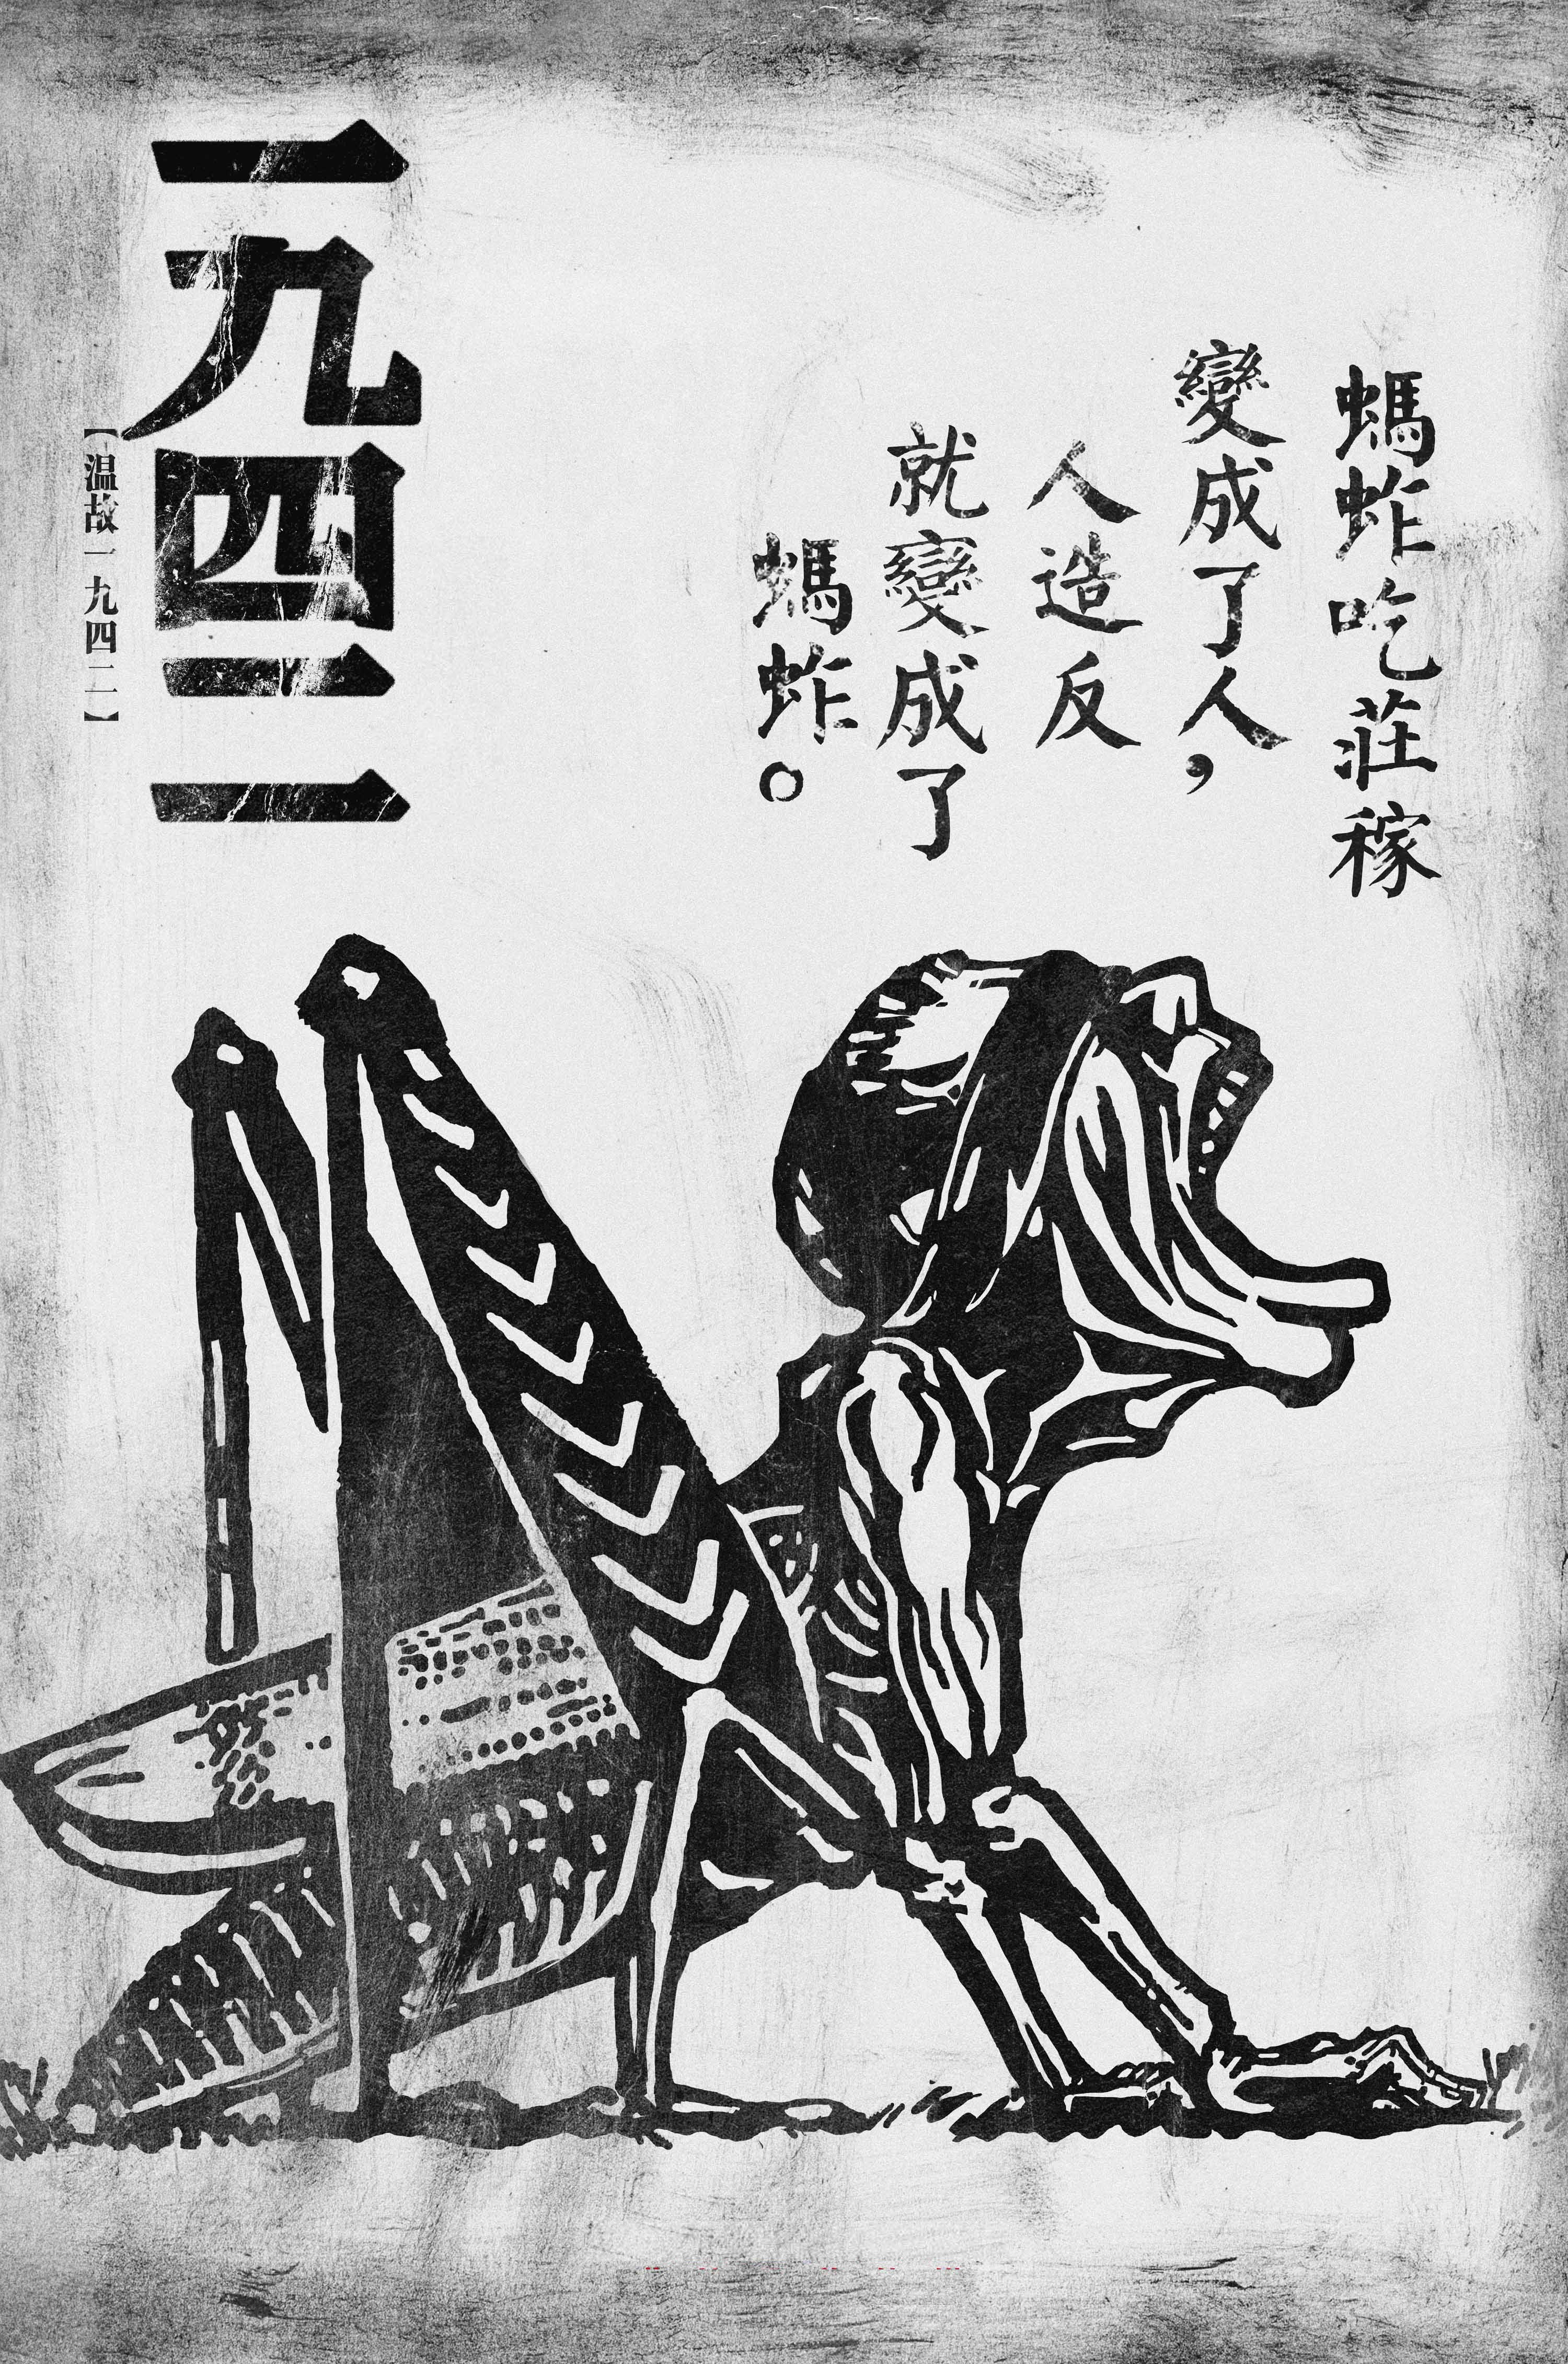
\includepdf[width=\paperwidth,height=\paperheight]{Frontmatter.jpg}
		\end{center}
	\end{figure}
	\newpage
	\begin{center}
		\phantom {placeholder}
	\vspace{5cm}
	{\Huge 温故一九四二}\\
	\vspace{2cm}
	{\Huge 刘震云}
	\end{center}
	\newpage
	{\color{TEXTColor}
		\begin{multicols}{2}
			\tableofcontents
		\end{multicols}
		\newpage
		\mainmatter
		\begin{multicols}{2}
			\fancyhead[LO]{{\scriptsize 【温故一九四二】序}} %奇數頁眉的左邊
\fancyhead[RO]{\thepage} %奇數頁眉的右邊
\fancyhead[LE]{\thepage} %偶數頁眉的左邊
\fancyhead[RE]{{\scriptsize 【温故一九四二】序}} %偶數頁眉的右邊
\fancyfoot[LE,RO]{}
\fancyfoot[LO,CE]{}
\fancyfoot[CO,RE]{}
\chapter*{序}
\addcontentsline{toc}{chapter}{\hspace{11mm}序}
%\thispagestyle{empty}
一九四二年,河南发生大灾荒。一位我所敬重的朋友,用一盘黄豆芽和两只猪蹄,把我打发回了一九四二年。当然,这顿壮行的饭,如果放到一九四二年,可能是一顿美味佳肴;同时就是放到一九四二年,也不见得多么可观。一九四三年二月,美国《时代》周刊记者白修德、英国《泰晤士》报记者哈里逊·福尔曼去河南考察灾情,在母亲煮食自己婴儿的地方,我故乡的省政府官员,宴请两个外国友人的菜单是:莲子羹、胡椒辣子鸡、栗子炖牛肉、豆腐、鱼、炸春卷、热馒头、米饭、两道汤,外加三个撒满了白糖的馅饼。这饭就是放到今天,我们这些庸俗的市民,也只能在书中和大饭店的菜本上看到。白修德说:这是他所吃过的最好的筵席之一。我说:这是我看到的最好的筵席之一。但他又说:他不忍心吃下去。我相信我故乡的省政府官员,决不会像白修德这么扭扭捏捏。说到底,一九四二年至一九四三年,我故乡发生了吃的问题。但吃的问题应该仅限在我们这些普通的百姓身上。我估计在我们这个东方文明的古国,无论发生什么情况,县以上的官员,都不会发生这种问题。不但不存在吃的问题,性的问题也不会匮乏。\\

还有一个问题,当我顺着枯燥泛出霉尿味的隧道回到一九四二年时,我发现五十年后我朋友把他交给我的任务的重要性,人为地夸大了。吃完豆芽和猪蹄,他是用一种上校的口气,来说明一九四二年的。\\

一九四二年夏到一九四三年春,河南发生大旱灾,景象令人触目惊心。全省夏秋两季大部绝收。大旱之后,又遇蝗灾。灾民五百万,占全省人口的百分之二十。“水旱蝗汤”,袭击全省一百一十个县。\\

灾民吃草根树皮,饿殍遍野。妇女售价累跌至过去的十分之一,壮丁售价也跌了三分之一。寥寥中原,赤地千里,河南饿死三百万人之多。\\

死了三百万。他严肃地看着我。我心里也有些发毛。但当我回到一九四二年时,我不禁哑然失笑。三百万人是不错,但放在当时的历史环境中去考察,无非是小事一桩。在死三百万的同时,历史上还发生着这样一些事:宋美玲访美、甘地绝食、斯大林格勒大血战、丘吉尔感冒。这些事件中的任何一桩,放到一九四二年的世界环境中,都比三百万要重要。五十年之后,我们知道当年有丘吉尔、甘地、仪态万方的宋美龄、斯大林格勒大血战,有谁知道我的故乡还因为旱灾死过三百万人呢?当时中国国内形势,国民党、共产党、日军、美国人、英国人、东南亚战场、国内正面战场、陕甘宁边区,政治环境错综复杂,如一盆杂拌粥相互搅和,摆在国家最高元首蒋介石委员长的桌前。别说是委员长,换任何一个人,处在那样的位置,三百万人肯定不是他首先考虑的问题。三百万是三百万人自己的事。所以,朋友交给我的任务是小节而不是大局,是芝麻而不是西瓜。当时世界最重要的部分是白宫、唐宁街十号、克里姆林宫、希特勒的地下掩体指挥部、日本东京,中国最重要的部分是重庆黄山官邸。这些富丽堂皇地方中的衣着干净、可以喝咖啡洗热水澡的少数人,将注定要决定世界上大多数人的命运。但这些世界的轴心我将远离,我要蓬头垢面地回到赤野千里、遍地饿殍的河南灾区。这不能说明别的,只能说明我从一九四二年起,就注定是这些慌乱下贱的灾民的后裔。最后一个问题是:朋友在为我壮行时,花钱买了两只猪蹄。匆忙之中,他竟忘记拔下盘中猪蹄的蹄甲;我吃了带蹄甲的猪蹄,就匆匆上路;可见双方是多么大意。\\
			\fancyhead[LO]{{\scriptsize 【温故一九四二】第一章}} %奇數頁眉的左邊
\fancyhead[RO]{\thepage} %奇數頁眉的右邊
\fancyhead[LE]{\thepage} %偶數頁眉的左邊
\fancyhead[RE]{{\scriptsize 【温故一九四二】第一章}} %偶數頁眉的右邊
\fancyfoot[LE,RO]{}
\fancyfoot[LO,CE]{}
\fancyfoot[CO,RE]{}
\chapter*{一}
\addcontentsline{toc}{chapter}{\hspace{11mm}第一章}
%\thispagestyle{empty}
我姥娘将五十年前饿死人的大旱灾,已经忘得一乾二净。我说:\\

“姥娘,五十年前,大旱,饿死许多人!”\\

姥娘:\\

“饿死人的年头多得很,到底指的哪一年?”\\

我姥娘今年九十二岁。与这个世纪同命运。这位普通的中国乡村妇女,解放前是地主的雇工,解放后是人民公社社员。在她身上,已经承受了九十二年的中国历史。没有千千万万这些普通的肮脏的中国百姓,波澜壮阔的中国革命和共产党历史都是白扯。他们是最终的灾难和成功的承受者和付出者。但历史历来与他们无缘,历史只漫步在富丽堂皇的大厅。所以俺姥娘忘记历史一点没有惭愧的脸色。不过这次旱灾饿死的是我们身边父老乡亲,是自己人,姥娘的忘记还是稍稍有些不对。姥娘是我的救命恩人。这牵涉到另一场中国灾难{\Add ──}一九六零年。老人家性情温和,虽不识字,却深明大义。我总觉中国所以能发展到今天,仍给人以信心,是因为有这些性情温和、深明大义的人的存在而不是那些心怀叵测、并不善良的人的生存。值得我欣慰的是,仗着一位乡村医生,现在姥娘身体很好,记忆力健全,我母亲及我及我弟弟妹妹小时候的一举一动,仍完整地保存在她的记忆里。我相信她对一九四二年的忘却,并不是一九四二年不触目惊心,而是在老人家的历史上,死人的事确是发生得太频繁了。指责九十二年许许多多的执政者毫无用处,但在哪位先生的执政下他的黎民百姓经常、到处被活活饿死,这位先生确应比我姥娘更感到惭愧。这个理应惭愧的前提是;他的家族和子孙,决没有发生饥饿。当我们被这样的人统治着时,我们不也感到不放心和感到后怕吗?但姥娘平淡无奇的语调,也使我的激动和愤怒平淡起来,露出自嘲的微笑。历史从来是大而化之的。历史总是被筛选和被遗忘的。谁是执掌筛选粗眼大筐的人呢?最后我提起了蝗虫。一九四二年的大旱之后,发生了遮天蔽日的蝗虫。这一特定的标志,勾起了姥娘并没忘却的蝗虫与死人的联系。她马上说:\\

“这我知道了。原来是飞蚂蚱那一年。那一年死人不少。蚂蚱把地里的庄稼都吃光了。牛进宝他姑姑,在大油坊设香坛,我还到那里烧过香!”\\

我说:\\

“蚂蚱前头,是不是大旱?”\\

她点着头:\\

“是大旱,是大旱,不大旱还出不了蚂蚱。”\\

我问:\\

“是不是死了很多人?”\\

她想了想:\\

“有个几十口吧。”\\

这就对了。一个村几十口,全省算起来,也就三百万了。我问:\\

“没死的呢?”\\

姥娘:\\

“还不是逃荒。你二姥娘一股人,三姥娘一股人,都去山西逃荒了。”\\

现在我二姥娘、三姥娘早已经不在了。二姥娘死时我依稀记得,一个黑漆棺材;三姥娘死时我已二十多岁,记得是一颗苍白的头,眼瞎了,像狗一样蜷缩在灶房的草铺上。他的儿子我该叫花爪舅舅的,在村里当过二十四年支书,从一九四八年当到一九七二年,竟没有治下一座象样的房子,被村里人嘲笑不已。放下二姥娘三姥娘我问:\\

“姥娘,你呢?”\\

姥娘:\\

“我没有逃荒。东家对我好,我又去给东家种地了。”\\

我:\\

“那年旱得厉害吗?”\\

姥娘比着:\\

“怎么不厉害,地裂得像小孩子嘴。往地上浇一瓢水,‘滋滋’冒烟。”\\

这就是了。核对过姥娘,我又去找花爪舅舅。花爪舅舅到底当过支书,大事清楚,我一问一九四二年,他马上说:\\

“四二年大旱!”\\

我:\\

“旱成甚样?”\\

他吸着我的“阿诗玛”烟说:\\

“一入春就没下过雨,麦收不足三成,有的地块颗粒无收;秧苗下种后,成活不多,活的也长尺把高,结不成籽。”\\

我:\\

“饿死人了吗?”\\

他点头:\\

“饿死几十口。”\\

我:\\

“不是麦收还有三成吗?怎么就让饿死了?”\\

他瞪着我:\\

“那你不交租子了?不交军粮了?不交税赋了?卖了田也不够纳粮,不饿死也得让县衙门打死!”\\

我明白了。我问:\\

“你当时有多大?”\\

他眨眨眼:\\

“也就十五六岁吧。”\\

我:\\

“当时你干什么去了?”\\

他:\\

“怕饿死,随俺娘到山西逃荒去了。”\\

撇下花爪舅舅,我又去找范克俭舅舅。一九四二年,范克俭舅舅家在我们当地是首屈一指的大户人家。我姥爷姥娘就是在他家扛的长工。东家与长工,过从甚密;范克俭舅舅几个月时,便认我姥娘为干娘。俺姥娘说,一到吃饭时候,范克俭他娘就把范克俭交给我姥娘,俺姥娘就把他放到裤腰里。一九四九年以后,主子长工的身份为之一变。俺姥娘家成了贫农,范克俭舅舅的爹在镇反中让枪毙了,范克俭舅舅成了地主分子,一直被管制到一九七八年。他的妻子、我的金银花舅母曾向我抱怨,说她嫁到范家一天福没享,就跟着受了几十年罪,图个啥呢?因为她与范克俭舅舅结婚于一九四八年底。但在几十年中,我家与范家仍过从甚密。范克俭舅舅见了俺姥娘就“娘、娘”地喊。我亲眼见俺姥娘拿一块月饼,像过去的东家对她一样,大度地将月饼赏给叫“娘”的范克俭舅舅。范克俭舅舅脸上露出感激的笑容。我与范克俭舅舅,坐在他家院中一棵枯死的大槐树下(这颗槐树,怕是一九四二年就存在吧?)共同回忆一九四二年。一开始范克俭舅舅不知一九四二年为何物,“一九四二年?一九四二年是哪一年?”这时我想起他是前朝贵族,不该提四九年以后实行的公元制,便说是民国三十一年。谁知不提民国三十一年还好些,一提民国三十一年范克俭舅舅暴跳如雷:\\

“别提民国三十一年,三十一年坏得很。”\\

我吃惊:\\

“三十一年为什么坏?”\\

范克俭舅舅:\\

“三十一年俺家烧了一座小楼!”\\

我不明白:\\

“为什么三十一年烧小楼?”\\

范克俭舅舅:\\

“三十一年不是大旱吗?”\\

我答:\\

“是呀,是大旱!”\\

范克俭舅舅:\\

“大旱后起蚂蚱!”\\

我:\\

“是起了蚂蚱!”\\

范克俭舅舅:\\

“饿死许多人!”\\

我:\\

“是饿死许多人!”\\

范克俭舅舅将手中的“阿诗玛”烟扔了一丈多远:\\

“饿死许多人,剩下没饿死的穷小子就滋了事。挑头的是毋得安,拿着几把大铡、红缨枪,占了俺家一座小楼,杀猪宰羊,说要起兵,一时来俺家吃白饭的有上千人!”\\

我为穷人辩护:\\

“他们也是饿得没办法!”\\

范克俭舅舅:\\

“饿得没办法,也不能抢明火呀!”\\

我点头:\\

“抢明火也不对,后来呢?”\\

范克俭舅舅诡秘地一笑:\\

“后来,后来小楼起了大火,麻杆浸着油。毋得安一帮子都活活烧死了,其它就做鸟兽散!”\\

“唔。”\\

是这样。大旱。大饥。饿死人。盗贼蜂起。\\

与范克俭舅舅分手,我又与县政协委员、四九年之前的县书记坐在一起。这是一个高大的、衰败的、患有不住摆头症的老头。虽然是县政协委员,但衣服破旧,上衣前襟上到处是饭点和一片一片的油渍。虽是四合院,但房子破旧,瓦檐上长满了枯黄的杂草。还没问一九四二年,他对他目前的境况发了一通牢骚。不过我并不觉得这牢骚多么有理,因为他的鼎盛时期,是四九年之前当县书记的时候。不过那时的县书记,不能等同于现在的县委书记,现在的县委书记是全县上百万人的父母官,那时的县书记只是县长的一个笔录,何况那时全县仅二十多万人。不过当我问起一九四二年,他马上不发牢骚了,立即回到了年轻力壮的鼎盛时期,眼里发出光彩,头竟然也不摇了。说:\\

“那时方圆几个县,我是最年轻的书记,仅仅十八岁!”\\

我点头。说:\\

“韩老,据说四二年大旱很厉害?”\\

他坚持不摇头说:\\

“是的,当时有一场常香玉的赈灾义演,就是我主持的。”\\

我点头。对他佩服。因为在一九九一年,中国南方发水灾,我从电视上见过赈灾义演。我总觉得把那么多鱼龙混杂的演艺人集合在一起,不是件容易的事。没想到当年的赈灾义演,竟是他主持的。接着老人家开始叙述当时的义演盛况及他的种种临时抱佛脚的解决办法。边说边发出爽朗开心的笑声。等他说完,笑完,我问:\\

“当时旱象如何?”\\

他:\\

“旱当然旱,不旱能义演?”\\

我绕过义演,问:\\

“听说饿死不少人,咱县有多少人?”\\

他开始摇头,左右频繁而有节奏地摇摆。摆了半天说:\\

“总有个几万人吧。”\\

看来他也记不清了。几万人对于当时的笔录书记,似也没有深刻的记忆。我告别他及义演,不禁长出一口气,也像他一样摇起头来。\\

这是在我故乡河南延津县所进行的旱情采访。据河南省志载,延津也是当时旱灾最严重的县份之一。但我这些采访都是零碎的,不完全、不准确的,五十年后,肯定夹杂了许多当事人的记忆错乱和本能的按个人兴趣的添枝或减叶。这不必认真。需要认真的,是当时《大公报》重庆版驻河南的战场记者高峰的一篇报道。这篇报道采访于当年,发表于当年,真实可靠性起码比我的同乡更真实可靠一些。这篇报道的标题是:《豫灾实录》。里边不但描写了旱灾与饥饿,还写到饥饿的人们在灾难里吃的是什么。这使我深深体会到,翻阅陈旧的报纸比到民间采访陈旧的年头便当多了。我既能远离灾难,又能吃饱穿暖居高临下地对灾难中的乡亲给予同情。\\

这篇报道写于一九四三年一月十七日。\\

\begin{quote}
	\begin{description}
		\item [$\bigtriangleup$] 记者首先告诉读者,今日的河南已有成千成万的人正以树皮(树叶吃光了)与野草维持着那可怜的生命。“兵役第一”的光荣再没有人提起,“哀鸿遍野”不过是吃饱穿暖了的人们形容豫灾的凄楚字眼。\\

		\item [$\bigtriangleup$] 河南今年(指旧历,乃是一九四二年)大旱,已用不着我再说。“救济豫灾”这伟大的同情,不但中国报纸,就是同盟国家的报纸也印上了大字标题。我曾为这四个字“欣慰”,三千万同胞也引颈翘望,绝望了的眼睛又发出了希望的光。希望究竟是希望,时间久了,他们那饿陷了的眼眶又葬埋了所有的希望。\\

		\item [$\bigtriangleup$] 河南一百十县(连沦陷县份在内),遭灾的就是这个数目,不过灾区有轻重而已,兹以河流来别:临黄河与伏牛山地带为最重,洪河汝河及洛河流域次之,唐河淮河流域又次之。\\

		\item [$\bigtriangleup$] 河南是地瘠民贫的省份,抗战以来三面临敌,人民加倍艰苦,偏在这抗战进入最艰难阶段,又遭天灾。今春(指旧历)三四月间,豫西遭雹灾,遭霜灾,豫南豫中有风灾,豫东有的地方遭蝗灾。入夏以来,全省三月不雨,秋交有雨,入秋又不雨,大旱成灾。豫西一带秋收之荞麦尚有希望,将收之际竟一场大霜,麦粒未能灌浆,全体冻死。八九月临河各县黄水溢堤,汪洋泛滥,大旱之后复遭水淹,灾情更重,河南就这样变成人间地狱了。\\

		\item [$\bigtriangleup$] 现在树叶吃光了,村口的杵臼,每天有人在那里捣花生皮与榆树皮(只有榆树皮能吃),然后蒸着吃。在叶县,一位小朋友对我说:“先生,这家伙刺嗓子!”\\

		\item [$\bigtriangleup$] 每天我们吃饭的时候,总有十几二十几个灾民在门口鹄候号叫求乞。那些菜绿的脸色,无神的眼睛,叫你不忍心去看,你也没有那些剩饭给他们。\\

		\item [$\bigtriangleup$] 今天小四饥死了,明天又听说友来吃野草中毒不起,后天又看见小宝冻死在寨外。可怜那些还活泼乱跳的下一代,如今都陆续的离开了人间。\\

		\item [$\bigtriangleup$] 最近我更发现灾民每人的脸都浮肿起来,鼻孔与眼角发黑。起初我以为是因饿而得的病症。后来才知是因为吃了一种名叫“霉花”的野草中毒而肿起来。这种草没有一点水分,磨出来是绿色,我曾尝试过,一股土腥味,据说猪吃了都要四肢麻痹,人怎能吃下去!灾民明知是毒物,他们还说:“先生,就这还没有呢!我们的牙脸手脚都是吃得麻痛!”现在叶县一带灾民真的没有“霉花”吃,他们正在吃一种干柴,一种无法用杵臼捣碎的干柴,所好的是吃了不肿脸不麻手脚。一位老夫说:“我做梦也没有想到吃柴火!真不如早死。”\\

		\item [$\bigtriangleup$] 牛早就快杀光了,猪尽是骨头,鸡的眼睛都饿得睁不开。\\

		\item [$\bigtriangleup$] 一斤麦子可以换二斤猪肉,三斤半牛肉。\\

		\item [$\bigtriangleup$] 在河南已恢复了原始的物物交换时代。卖子女无人要,自己的年轻老婆或十五六岁的女儿,都驮到驴上到豫东驮河、周家口、界首那些贩人的市场卖为娼妓。卖一口人,买不回四斗粮食。麦子一斗九百元,高粱一斗六百四十九元,玉米一斗七百元,小米十元一斤,蒸馍八元一斤,盐十五元一斤,香油也十五元。没有救灾办法,粮价不会跌落的,灾民根本也没有吃粮食的念头。老弱妇孺终日等死,年轻力壮者不得不铤而走险,这样下去,河南就不需要救灾了,而需要清乡防匪,维持地方的治安。\\

		\item [$\bigtriangleup$] 严冬到了,雪花飘落,灾民无柴无米无衣无食,冻馁交迫。那薄命的雪花正象征着他们的命运。救灾刻不容缓了。\\
	\end{description}
\end{quote}

			\fancyhead[LO]{{\scriptsize 【温故一九四二】第二章}} %奇數頁眉的左邊
\fancyhead[RO]{\thepage} %奇數頁眉的右邊
\fancyhead[LE]{\thepage} %偶數頁眉的左邊
\fancyhead[RE]{{\scriptsize 【温故一九四二】第二章}} %偶數頁眉的右邊
\fancyfoot[LE,RO]{}
\fancyfoot[LO,CE]{}
\fancyfoot[CO,RE]{}
\chapter*{二}
\addcontentsline{toc}{chapter}{\hspace{11mm}第二章}
%\thispagestyle{empty}
重庆黄山官邸。这里生机盎然,空气清新,一到春天就是满山的桃红和火焰般的山茶花。自南京陷落以后,国民政府迁都重庆,这里是蒋介石委员长的住处。当时蒋在重庆有四处官邸,这是其中之一。领袖的官邸,与国家沦陷、国家强弱没有关系;这里既不比南京的几处官邸差,也不比美国的白宫、英国的唐宁街十号逊色。领袖总是领袖,只要能当上领袖,不管当上什么肤色、民族的领袖,都可以享受到世界一流的衣、食、住、行。虽然所统治的民众大相径庭。所以,我历来赞成各国领袖之间握手言欢,因为他们才是真正的阶级兄弟;各国民众之间,既不必联合,也没有什么可说的。即使发生战争,也不可怕,世界上最后一颗炮弹,才落在领袖的头上。如果发生世界性的核战争,最后剩下的,就是各国的几位领袖,因为他们这时住在风景幽美的地球上空,掌握着核按钮。掌握按纽的人,历来是不会受伤害的。黄山官邸以云岫楼和松厅为中心结构,蒋住云岫楼,仪态万方的宋美龄住松厅。当然,夜间就难说了,如果两人有兴致的话。在两处住宅之间的低谷里,专门挖有防空洞,供蒋、宋躲他们阶级兄弟日本天皇陛下的飞机。至于蒋、宋的日常生活,这不是我们所能想象的,反正整日的吃喝,比五十年后我们十二亿人中的十一亿九千九百九十九万人还要好,还要不可想象。虽然蒋只喝白水,不饮酒、不抽烟、安假牙,信基督,但他也肯定知道,榆树皮和“霉花”,是不可吃的,可吃的是西餐和中餐中的各种菜系。一九四二年,蒋与他的参谋长、美国人史迪威发生矛盾,在黄山官邸吵嘴,即要不欢而散,宋美龄挽狂澜于即倒,美丽地笑着说:“将军,都是老朋友了,犯不着这样怄气。要是将军能赏光到我的松厅别墅去坐一坐,将会喝到可口的咖啡!”\\

这是我在一本书上读到的。读到这里,我对他们吵不吵嘴并不感兴趣,反正吵嘴的双方都已经去球了,不在这个世界上了。我注意到:一九四二年,中国还是有“可口的咖啡”,虽然我故乡的人民在吃树皮、柴火、稻草和使人身体中毒发肿的“霉花”,最后饿死三百万人。当然,这样来故意对比,说明我这个人无聊,把什么事情都弄得庸俗化。我也知道,对一个泱泱大国政府首脑的要求,不在他的夫人有无有咖啡,只要他们每天不喝人血(据说中非的皇帝就每天喝人血),无论喝什么,吃什么,只要能把国家治理好,就是一个民族英雄和历史伟人。我在另一本书上看到,蒋为了拉拢一部地方武装,对戴笠说:“你去办一办。记住,多花几个钱没关系。”这钱从何而来呢?我只是想说,一九四二年,当我故乡发生大旱灾、大饥饿的消息传到黄山官邸时,蒋委员长对这消息不该不相信。当然,也不是不信,也不是全信,他说:可能有旱灾,但情况不会这么严重。他甚至怀疑是地方官员虚报灾情,像军队虚报兵员为了吃空额一样,想多得一些救济粮和救济款。蒋委员长的这种态度,在几十年后的今天,受到许多书籍的指责。他们认为委员长不体察民情、不爱民如子、固执等。他们这种爱民如子、横眉冷对民贼独夫的态度,也感染了我的情绪。但当我冷静下来,我又是轻轻一笑。这时我突然明白,该受指责的不是委员长,而是几十年后这些书的自作聪明的作者。是侍从在梦中,还是丞相在梦中?侍从在梦中。不设身处地,不身居高位,怎么能理解委员长的心思?书籍的作者,不都是些百无一用的书生吗?委员长是委员长都当上了,头脑不比一个书生聪明?是书生领导委员长,还是委员长领导书生?是委员长见多识广,还是书生见多识广?一切全在委员长{\Add ──}万般世界,五万万百姓,皆在委员长心中。只是,当时的委员长的所思所想,高邈深远,错综复杂,并不被我们所理解。委员长真不相信河南有大旱灾、旱灾会饿死人吗?非也。因为从委员长的出身考察,相对于宋美龄小姐来说,委员长还算是苦出身。委员长自己写道:\\

我九岁丧父……。当时家里的悲惨情况实在难以形容。我家无依无靠,没有势力,很快成了大家污辱和虐待的对象。\\

这样一个出身的人,不会不知道下层大众所遭受的苦难。在一个省的全部范围内发生了大旱灾,情况严重到什么程度,他心里不会没底。但他认为:可能有旱灾,但不会这么严重。于是书生们上了当,以为委员长是官僚主义。其实在梦中的是书生,清醒的是委员长。那么为什么心里清楚说不清楚呢?明白情况严重而故意说不严重呢?这是因为摆在他面前的,有更多的,比这个旱灾还严重的混沌不清需要他理清楚处理妥当以致不犯历史错误的重大问题。须知,在东方饿死三百万人不会影响历史。\\

这时的委员长,已不是一个乡巴佬,而是一个领袖。站在领袖的位置上,他知道轻重缓急。当时能导致历史向不同方向发展的事情大致有:\\

\begin{quote}
	\begin{description}
		\item [一、] 	中国的同盟国地位问题。当时同盟国有美、英、法、苏、中等。蒋虽是中国的领袖,但同盟国的领袖们坐在一起开会,如开罗会议,蒋就成了一个普通人,成了一个小弟兄,成了一个无足轻重的人。大家在一起,似乎罗斯福、丘吉尔、斯大林,都不把蒋放在眼里。不把蒋放眼里,就是不把中国放到眼里。由此以来,在世界战局的分布上,中国就常常是战略的受害者。而中国最穷,必须在有外援的情况下才能打这场战争,所以常常受制于人,吃哑巴亏;带给蒋个人的,就是仍受“侮辱和虐待”。这是他个人心理上暗自痛恨的。\\
		
		\item [二、] 	对日战争问题。在中国正面战场,蒋的军队吸引了大部分在华日军,虽然不断丢失土地,但从国际战略上讲,这种牵制本身,就给其它同盟国带来莫大的利益;但同盟国其它领袖并没认清这一点或是认清了这一点而故意欺辱人,所给的战争物资,与国民党部队所担负的牵制任务,距离相差非常大;从国内讲,国民党部队在正面战场牵制日军,使得共产党在他的根据地得到休养生息,这是蒋的心腹大患,于是牵涉到了对共产党的方针。蒋有一著名的理论,“攘外必先安内”。这口号从民族利益上讲,是狭隘的,容易激起民愤的;如果从蒋的统治利益出来,又未尝不是一个统治者必须采取的态度。如只是攘外,后方的敌人发展起来,不是比前方的敌人更能直捣心脏吗?关于这一方针,他承受着巨大的国际、国内压力。\\
		
		\item [三、] 	国民党内部、国民政府内部各派系的斗争。蒋曾很后悔地说:北伐战争之后,他不该接受那么多军阀部队;一九四九年后说:我不是被共产党打倒的,我是被国民党打倒的;可见平日心情。四、他与他的参谋长{\Add ──}美军上将史迪威将军,发生了严重的战略上和个人间的矛盾,这牵涉到对华援助和蒋个人在美国的威信问题。史迪威已开始在背后不体面地称这位中国民族的领袖为“花生米”{\Add ──}以上所有这些问题,包括一些我们还没觉察到而蒋在他的位置上已经觉察到的问题,都有可能改变历史的方向和写法,这时,出现了一个地方省(当时全国三十多个省)的旱灾,显得多么无足轻重。死掉一些本就无用、是社会负担的老百姓,不会改变历史的方向;而他在上层政治的重大问题上处理稍有不慎,历史就可能向不利于他的方向发展,后来一九四五年至一九四九年,就证明了这一点。上述哪一个重大问题,对于一个领袖来讲,都比三百万人对他及他的统治地位影响更直接,更利益交关。从历史地位上说,三百万人确没有一粒“花生米”重要。所以,他心里清楚旱灾,仍然要说:可能有旱灾,但不会那么严重。于是他厌恶那些把他当傻瓜当官僚以为他不明真相而不厌其烦向他提供真情况的人,特别是那些爱管闲事、爱干涉他国内政的外国人。这就是蒋委员长此时此刻的心境。当然,这是站在蒋的立场上考察问题;如果换一个角度,当我们站在几千万灾民的立场上去考察,就觉得蒋无疑是独夫民贼,置人民的生死于不顾了。\\
	\end{description}
\end{quote}

世界有这样一条真理,一旦与领袖相处,我们这些普通的百姓就非倒霉不可。蒋的这种态度,使受灾的几千万人只有吃树皮、稻草、干柴和“霉花”,而得不到一个政府所应承担的救济,调剂和帮助。于是,人口在大面积死亡。但这不是事情最重要的部分,事情最重要的部分是:\\

在大面积受灾和饿死人的情况下,政府向这个地区所征的实物税和军粮任务不变。\\

陈布雷说:\\

委员长根本不相信河南有灾,说是省政府虚报灾情。李主席(培基,河南省政府主席)的报灾电,说什么“赤地千里”,“哀鸿遍地”“嗷嗷待哺”等等,委员长就骂是谎报滥调,并且严令河南的征实不能缓免。\\

这实际等于政府又拿了一把刀子,与灾害为伍,在直接宰杀那些牲口一样的两眼灰蒙蒙、东倒西歪的灾民。于是,死的死了;没死的,发生大面积背井离乡的逃荒。五十年后的今天,我们也会像蒋委员长那样说:情况不会那么严重吧?这是一种事物的惯性,事物后特别过很长一段时间后再来想事物,我们总是宽宏大量地想:事情不会那么严重吧?但在当时,可知历史是一点不宽容的。为了证明这一点,我们又得引用资料。我认为这种在历史中打捞事件的报告式的文字,引用资料比作者胡编乱造要更科学一些。后者虽然能使读者身临其境,但其境是虚假的;资料也可能虚假,但五十年前的资料,总比五十年后的想象更真实一些。一九四二年,美国驻华外交官约翰·S·谢伟思在给美国政府的报告中写道:\\

河南灾民最大的负担是不断加重的实物税和征收军粮。由于在中条山失陷之前,该省还要向驻守山西南部的军队和驻守在比较穷困的陕西省的军队提供给养,因而,负担也就更加沉重了。在陕西省的四十万驻军的主要任务是“警戒”共产党。\\

我从很多人士那里得到的估计是:全部所征粮税占农民总收获的百分之三十至五十,其中包括地方政府的征税,全国性的实物土地税(通过省政府征收)以及形形色色、无法估计的军事方面的需求。税率是按正常的年景定,而不是按当年的实际收成定。因此,收成越坏,从农民征收的比例就越大。征粮要缴纳小麦,因此,他们所收获的小麦更大一部分要用于纳粮。\\

有很可靠的证据表明,向农民征收的军粮是超过实际需要的。中国军官的一个由来已久的,仍然盛行不衰的惯例,就是向上级报告的部队人数超过实际所有的人数。这样他们就可以吃空额,谋私利。洛阳公开市场上的很大一批粮食,就是来自这个方面……\\

人们还普遍抱怨,征粮征税负担分配不公平。这些事是通过保甲长来办,他们自己就是乡绅、地主。他们通常都是要使自己和他们的亲朋好友不要纳粮纳税太多。势力还是以财富和财产为基础:穷苦农民的粮食,往往被更多地征去了,这就正像是他们的儿子,而不是甲长和地主的儿子,被拉去当兵一样。\\

河南的情况是如此之糟,以致在好几年中都有人逃荒到陕西、甘肃和川北……。结果是河南的人口相对减少,而留下来的,人和赋税负担相对加重了。在前线地区,农民的日子最苦,那里受灾也最重。因此,来自那里的人口流动也最多。来自郑州的一位传教士说,早在当年的饥荒袭来之前,那个地区的许多田园就已荒无人烟了。\\

这种情况今年发展到了顶点。最盲目的政府官员也认识到,在小麦欠收后,早春将发生严重缺粮。早在七月间,每天就有约一千名难民逃离河南,但是,征粮计划不变。在很多地区,全部收成不够纳粮的需要。在农村发生了一些抗议,但都是无力的,分散的,没有效果的。在少数地方,显然使用了军队对付人民。吃着榆树皮和干树叶的灾民,被迫把他们最后一点粮食种子交给税收机关。身体虚弱得几乎走不动路的农民还必须给军队交纳军马饲料。这些饲料比起他塞进自己嘴里的东西,其营养价值要高得多。\\

以上是谢伟思的报告。为什么我引用谢的文字而不引证别的书籍呢?因为谢是外国人,不身在复杂的其中,也许能更客观一些。但谢伟思所说的,还不是最严重的,即:在灾难中的灾民,并不被免除赋税,而是严令仍按正常年景税赋征收因而实际上税赋已超过正常年景还不是重要的,更重要的,是统治这些灾民的一些官员,还借灾民的灾难去投机发财。据美国记者白修德亲眼目睹,有些部队的司令把部队的余粮卖给实民,发了大财。来自西安和郑州的商人,政府的小官吏、军官以及仍然储蓄着粮食在手的地主,拼命以罪恶的低价收买农民祖辈留下来的田地。土地的集中和丧失同时进行,其激烈程度与饥饿的程度成正比。\\

当我们被这么一些从委员长一直到小官吏、地主所统治的时候,我们的命运操纵在他们手里,我们对他们的操纵能十分放心吗?\\

后来,就必然出现了大批的脱离了土地的灾民,出现一个由东向西的大规模的流民图。这流民中,就包括河南延建县王楼乡老庄的俺二姥娘、俺三姥娘全家,包括村里其它许多父老乡亲。他们虽然一辈子没有见过委员长,许多青壮年一听委员长还自觉立正,但是,委员长在富丽堂皇的黄山别墅的态度,一颦一笑,都将直接决定他们的生死和命运。委员长思索:中国向何处去?世界向何处去?他们思索,我们向哪里去逃荒?\\
			\fancyhead[LO]{{\scriptsize 【温故一九四二】第三章}} %奇數頁眉的左邊
\fancyhead[RO]{\thepage} %奇數頁眉的右邊
\fancyhead[LE]{\thepage} %偶數頁眉的左邊
\fancyhead[RE]{{\scriptsize 【温故一九四二】第三章}} %偶數頁眉的右邊
\fancyfoot[LE,RO]{}
\fancyfoot[LO,CE]{}
\fancyfoot[CO,RE]{}
\chapter*{三}
\addcontentsline{toc}{chapter}{\hspace{11mm}第三章}
%\thispagestyle{empty}
重庆黄山官邸。这里生机盎然,空气清新,一到春天就是满山的桃红和火焰般的山茶花。自花爪舅舅直到现在还有些后悔。当初在洛阳被抓了壮丁,后来为什么要逃跑,没有在部队坚持下来呢?我问:\\

“当时抓你的是哪个部队?”\\

花爪舅舅:\\

“国军。”\\

我:\\

“我知道是国军,国军的哪一部分?”\\

花爪舅舅:\\

“班长叫个李狗剩,排长叫个闫之栋。”\\

我:\\

“再往上呢?”\\

花爪舅舅:\\

“再往上就不知道了。”\\

我事后查了查资料,当时占据洛阳一带的国民党部队,隶属胡宗南。我问:\\

“被抓壮丁后干什么去了?”\\

花爪舅舅:\\

“当时就上了中条山,派到了前线。日本人的追击炮,‘啾啾’地在头上飞。打仗头一天,班副和两个弟兄就被炸死了。我害怕了,当晚就开溜了。现在想起来,真是后悔。”\\

我:\\

“是呀,大敌当前,民族矛盾,别的弟兄牺牲了,你开溜了,是不大象话,该后悔。”\\

花爪舅舅瞪我一眼:\\

“我不是后悔这个。”\\

我一愣:\\

“那你后悔什么?”\\

花爪舅舅:\\

“当初不开溜,后来跑到台湾,现在也成台胞了。像通村的王明芹,小名强驴,抓壮丁比我还晚两年,后来到了台湾,现在成了台胞,去年回来了,带着小老婆,戴着金壳手表,镶着大金牙,县长都用小轿车接他,是玩的不是?这不能怪别的,只能怪你舅眼圈子太小,年轻不懂事。当时我才十五六岁,只知道活命了。”\\

我明白了花爪舅舅的意思。我安慰他:\\

“现在后悔是对的,当初逃跑也是对的。你想,一九四三年,离抗日战争结束还有两年,以后解放战争还有五年,谁也难保证你在诸多的战斗中不像你们班副一样被打死。当然,如果不打死,就像强驴一样成了台胞;如果万一打死,不连现在也没有了。”\\

花爪舅舅想了想:\\

“那倒是,子弹没长眼睛;我就是这个命,咱没当台胞那个命。”\\

我说:\\

“你虽然没当台胞,但在咱们这边,你也当了支书,总起说混得还算不错。”\\

花爪舅舅立即来了精神:\\

“那倒是,支书我一口气当了二十四年!”\\

但马上又颓然叹口气:\\

“但是十个支书,加起来也不顶一个台胞呀。现在又下了台,县长认咱是谁呀。”\\

我安慰他:\\

“认识县长也没什么了不起,不就是一个强驴吗?舅舅,咱们不说强驴了,咱们说说,俺二姥娘一家、三姥娘一家,当初是怎么逃荒的,你身在其中,肯定有许多亲身经历。”\\

一说到正题,花爪舅舅的态度倒变得无所谓,叙述得也简单和枯燥了。两手相互抓着说:\\

“逃荒就是逃荒呗。”\\

我:\\

“怎么逃荒,荒怎么逃法?”\\

他:\\

“俺爹推着独轮车,俺二大爷挑着箩筐,独轮车上装些锅碗瓢盆,箩筐里挑些小孩。路上拉棍要饭,吃树皮,吃杂草。后来到了洛阳,我就被抓了兵。”\\

我不禁埋怨:\\

“你也说得太简单了,路上就没有什么现在还记得的事情?”\\

他眨眨眼:\\

“记得路边躺着睡觉特冷,半夜就冻醒了。见俺爹俺娘还在睡,也不敢说话。”\\

我:\\

“后来怎么抓的兵?”\\

他:\\

“洛阳有天主教办的粥场,我去挤着打粥,回来路上,就被抓了兵。”\\

我:\\

“抓兵俺三姥爷三姥娘知道不?”\\

他摇摇头:\\

“他们哪里知道?认为我被人拐跑了。再见面就是十年之后了。”\\

我点点头。又问:\\

“你抓兵他们怎么办?”\\

他:\\

“十年后我才听俺娘说,他们扒火车去陕西。扒火车时,俺爹差点让火车轧着。”\\

我:\\

“俺二姥娘家一股呢?”\\

他:\\

“你二姥爷家扒火车时,扒着扒着,火车就开了,把个没扒上来的小妹妹{\Add ──}你该叫小姨,也给弄失散了,直到现在没找见。”\\

我点点头。又问:\\

“路上死人多吗?”\\

他:\\

“怎么不多,到处是坟包,到处是死人。扒火车还轧死许多。”\\

我:\\

“咱家没有饿死的?”\\

他:\\

“怎么没有饿死的,你二姥爷,你三妗,不都是饿死在道儿上?”\\

我:\\

“就没有一些细节?”\\

这时花爪舅舅有些不耐烦了,愤怒地瞪我一眼:\\

“人家人都饿死了,你还要细节!”\\

说完,丢下我,独自蹶蹶地走了,把我扔在一片尴尬之中。这时我才觉得朋友把我打发回一九四二年真是居心不良,我在揭亲人和父老的已经愈合五十年的伤疤,让他们重新露出血淋淋的创面;何况这疤疖也结得太厚,被岁月和灰尘风干成了盔甲,搬动它像搬动大山一样艰难费劲。\\

没有风,太阳直射在一大溜麦秸垛上。麦秸垛旁显得很温暖。我蹲在麦秸垛旁,正费力地与一个既聋又瞎话语已经说不清楚且鼻涕流水的八十多岁的老人说话。老人叫郭有运。据县政协委员韩给我介绍,他是一九四三年大逃荒中家中受损失最重的一个。老婆、老娘、三个孩子,全丢在了路上。五年后他从陕西回来,已是孤身一人。现在的家庭,属于重起炉灶。但看麦秸垛后他重搭的又经营四十多年的新炉灶,证明他作为人的能力,还属上乘。因为那是我故乡乡村中目前还不常见的一幢不中不西的二层小楼。但如果从他年龄过大而房子很新的角度来考察,这不应算是他的能力,成绩应归功于坐在我们中间当翻译的留着分头戴着“戈尔巴乔夫”头像手表的四十岁的儿子。他的儿子一开始对我的到来并不欢迎,只是听说我与这个乡派出所的副所长是光屁股同学,才对我另眼相看。但听到我的到来与现实中的他没有任何关联,而是为了让他爹和我共同回到五十年前,而五十年前他还在风里云里飘,就又有些不耐烦。老人家的嘴漏风,呜里呜啦,翻译不耐烦,所得的五十年前的情况既生硬又零碎。我又一次深深体会到,在活人中打捞历史,实在不是一件容易的事。郭有运在一九四三年逃荒中的大致情况是:一上路,他娘就病了;为了给他娘冶病,卖掉一个小女;为卖这个小女,跟老婆打了一架。打架的原因不单纯是卖女心疼,而是老婆与婆婆过去积怨甚深,不愿为治婆婆的病卖掉自己的骨肉。卖了小女,娘的病也没治好,死在黄河边,软埋(没有棺材)在一个土窑里。走到洛阳,大女患天花,病死在慈善院里。扒火车去潼关,儿子没扒好,掉到火车轮下给轧死了。剩下老婆与他,来到陕西,给人拦地放羊。老婆嫌跟他生活苦,跟一个人拐子逃跑了。剩下他自己。麦秸垛前,他一把鼻涕一把泪地摊着手:\\

“我逃荒为个啥?我逃荒为图大家有个活命,谁知逃来逃去剩下我自己,我还逃荒干什么?早知这样,这荒不如不逃了,全家死还能死到一块,这死得七零八落的。”\\

这段话他儿子翻得很完全。我听了以后也感到是一个怪圈。我弄不明白的还有,现在不逃荒了,郭有运的新家有两层小楼,为什么还穿得这么破衣烂衫,仍像个逃荒的样子呢?如果不是老人家节俭的习惯,就是现实中的一切都不属于他。这个物质幸福的家庭,看来精神上并不愉快。这个家庭的家庭关系没有或永远没法理顺。我转过头对他儿子说:“老人家也不易,当年逃荒那个样子!”\\

谁知他儿子说:\\

“那怪他窝囊。要让我逃荒,我决不会那么逃!”\\

我吃了一惊:\\

“要让你逃,你怎么逃?”\\

他儿子:\\

“我根本不去陕西!”\\

我:\\

“你去哪儿?”\\

他儿子:\\

“我肯定下关东!关东不比陕西好过?”\\

我点头。关东肯定比陕西富庶,易于人活命。但我考察历史,我故乡没有向关东逃荒的习惯:闯关东是山东、河北人的事。我故乡遇灾遇难,流民路线皆是向西而不是往北。虽然西边也像他的故乡一样贫瘠。当然,一九四二、一九四三年还有一个特殊情况,就是东北三省已被日本人占了,去了是去当亡国奴。我把这后一条理由向他儿子谈了,谁知他一挥手上的“戈尔巴乔夫”,发出惊人论调:\\

“命都顾不住了,还管地方让谁占了?向西不当亡国奴,但他把你饿死了。换你,你是当亡国奴好呢,还是让饿死呢?不当亡国奴,不也没人疼你爱你管你吗?”\\

我默然,一笑。他提出的问题我解答不了。我想这是蒋委员长的失算,及他一九四九年逃到台湾的深刻原因。假如我处在一九四二年,我是找不管不闻不理不疼不爱我的委员长呢,还是找还能活命的东北关外呢?\\

告别郭有运和他的儿子,我又找到十李庄一位姓蔡的老婆婆。但这次采访更不顺利,还没等我与老婆婆说上话,就差点遭到她儿子的一顿毒打。姓蔡的婆婆今年七十岁,五十年前,也就二十岁。在随爹娘与两个弟弟向西逃荒时,路上夜里睡觉,全家的包袱、细软、盘缠、粮食,全部被人席卷一空。醒后发现,全家人只好张着傻嘴大哭。再向西逃没有活咱。她的爹娘只好把她卖掉,保全两个弟弟。一开始以为卖给了人家,但人贩子将她领走,转手又倒卖给窑子,从此做了五年皮肉生涯。直到一九四八年,国共两党的军队交战,隆隆炮声中,她逃出妓院,逃回家乡,像郭有运老汉一样,她现在的家庭、儿子、女儿一大家人,都是重起炉灶另建立的。她五年的肮脏非人生活,一直埋藏在她自己和大家的心底,除非邻里吵架时,被别的街坊娘们重新抖落一遍。但到了八十年代后期,她的这段生活,突然又显示出它特有的价值。本地的、外地的一些写畅销书的人,都觉得她这五年历史有特殊的现实意义,纷纷来采访她,要以她五年接客的种种情形,写出一本“我的妓女生涯”的自传体畅销书。从这题目看,畅销是必然的。为多写字的来采访,一开始使这个家庭很兴奋,原来母亲的经历还有价值,值得这些衣着干净人的关心。大家甚至感到很荣耀。但时间一长,当儿女们意识到写字的关心他们的目的,并不是为了关心他们自身,而是为了拿母亲的肮脏经历去为自己赚钱,于是她的儿女们,这些普普通通的庄稼人,突然感到自己受了骗,受了污辱。于是对再来采访的人,就怒目而视。为此,他们洋洋自得仍兴奋地沉浸在当年情形中的母亲,受到了她的儿子们严厉斥责。母亲从此对五十年前的事情又守口如瓶:已经说过的,也断然反悔。这使已经写下许多文字的人很尴尬。“我的妓女生涯”也因此夭折。这桩公案已经过去好几年了,现在我到这里来,又被她的儿子认为是来拿他母亲的肮脏经历赚钱的,要把已经夭折的“妓女生涯”再搭救起来。因此,我还没能与老婆婆说上话,他儿子的大棒,已差点落到我的头上。我不是一个多么勇敢的人,只好知难而退。而且我认为为了写这篇文章,去到处揭别人伤疤,特别是一个老女人肮脏的脓疮时,确实不怎么体面。我回去告诉了在乡派出所当副所长的我的小学同学,没想到他不这么认为,他怪我只是方式不对。他甩了甩手里的皮带说:\\

“这事你本来就应该找我!”\\

我:\\

“怎么,你对这人的经历很清楚?”\\

他:\\

“我倒也不清楚,但你要清楚什么,我把她提来审一下不就完了?”\\

我吃一惊,忙摆手:\\

“不采访也罢,用不着大动干戈。再说,她也没犯罪,你怎么能说提审就提审!”\\

他瞪大眼珠:\\

“她是妓女,正归我打击,我怎么不可以提审?”\\

我摆手:\\

“就是妓女,也是五十年前,提审也该那时的国民党警察局提审,也轮不到五十年后的你!”\\

他还不服气:\\

“五十年前我也管得着,看我把她抓过来!”\\

我忙拦住他,用话岔开,半天,才将气呼呼的他劝下。离开他时,我想,同学毕竟是同学呀。\\

为了把这次大逃荒记述下去,我们只好再次借助于《时代》周刊记者白修德。文章写到这里,我已清楚地意识到,白修德,必将成为这篇文章的主角,这不是因为别的,是因为一九四二年的河南大灾荒,已经没有人关心。当时的领袖不关心,政府不关心,各级官员在倒卖粮食发灾难财,灾民自己在大批死去,没死的留下的五十年后的老灾民,也对当年处以漠然的态度。这时,唯有一个外国人,《时代》周刊记者白修德,倒在关心着这片饥荒的土地和三百万饿死的人。自已的事情,自己这样的态度,自己的事情让别人关心、同情,说起来让五十年后的我都感到脸红。当然,白修德最初的目的,也不是为了关心我们的民众,他是出于一个新闻记者的敏感,要在大灾荒里找些可写的东西。无非是在找新闻的时候,悲惨的现实打动了他,震憾了他,于是产生了一个正常人的同情心,正义感,要为之一呼。这就有了以后他与蒋介石的正面冲突。说也是呀,一个美国人可以见委员长,有几个中国人,可以见到自己的委员长呢?怕是连政府的部长,也得事先预约吧。我们这些无依无靠的灾民,像自己父母一样的各级官员我们依靠不得,只好依靠一个其它力量并不强大的外国记者了。特别是后来,这种依靠也起了作用,这让五十年后的我深受震动、目瞪口呆。\\

白修德在一本《探索历史》的书中,描述了他一九四三年二月的河南之行。同行者是英国《泰晤士报》记者哈里林·福尔曼。在这篇文字开头我曾说到,在他们到达郑州时,曾在我的家乡吃过一顿“他能吃过的最好的筵席之一”。他们当时的行走路线是;从重庆飞抵宝鸡,剩陇海线火车从宝鸡到西安,到黄河,到潼关,然后进入河南。为防日本人炮击,从潼关换乘手摇的巡道车,整整一天,到达洛阳。所走的正是难民逃难的反方向。到达河南后,骑马到郑州,然后由郑州搭乘邮车返回重庆。从这行走路线看,是走马观花,只是沿途看到一些情形。记下的,都是沿途随时的所见所闻。这些所见是零碎的,所谈的见解带有很大的个人见识性。何况中美国情不同,这种个人见解离实际事务所包含的真正意蕴,也许会有一段距离。但我们可以为开这些见识,进入他的所见,进入细节;他肉眼看到的路边事实,总是真实的。我们可以根据这些真实的事实,去自己见识一九四三年的河南灾民大逃荒。我试图将他这些零碎的见闻能归纳得条理一些。\\

\begin{quote}
	\begin{description}
		\item [一、] 灾民的穿戴和携带。灾民逃出来时,穿的都是他们最好的衣服,中年妇女穿著红颜绿色的旧嫁衣,虽然衣服上已是污迹斑斑;带的是他们家中最有价值的东西,烧饭铁锅,铺盖,有的还有一座老式座钟。这证明灾民对自己的故乡已彻底失去信心,没有留恋,决心离开家乡热土,连时间{\Add ──}座钟都带走了。白修德与他的伙伴在潼关车站睡了一夜。他说,那里到处是尿臊味、屎臭味和人身上的臭味。为了御寒,许多人头上裹着毛巾,有的帽子把帽耳朵放下来。他们在这里的目的,是为了等待往西去的火车,虽然这种等待是十分盲目的。\\
		
		\item [二、] 逃荒方式。不外是扒火车和行走。扒火车很不安全。白修德说,他沿途见到许多血迹斑班的死者。一种是扒上了火车,因列车被日本人的炮弹炸毁而丧命;有的是扒上了车厢顶,因夜里手指冻僵,失去握力,自己从车厢顶摔下摔死的;还有的是火车没扒上,便被行走的火车轧死的。轧死还好些,惨的是那些轧上又没轧死的。白见到一个人躺在铁轨旁,还活着,不停地喊叫,他的小腿被轧断,腿骨像一段白色的玉米杆那样露在外面。他还见到一个臀部轧得血肉模糊还没死去的人。白修德说,流血并不使他难过,难过的是弄不明白这些景象究竟是怎么回事。这么无组织无纪律的迁徙,他们各级政府哪里去了?{\Add ──}这证明白修德太不了解中国国情了。扒不上火车或对火车失望的,便是依靠自己的双腿,无目的无意识地向西移动。白修德说,整整一天,沿着铁路线,“我见到的便是这些由单一的、一家一户所组成的成群结队一眼望不到头的行列。”这种成群结队是自发的、无组织的,只是因为饥荒和求生的欲望,才使他们自动地组成了灾民的行列。可以想象,他们的表情是漠然的,他们也不知道,前边等待他们的是什么。唯一留在心中的信心,便是他们自己心中对前方未来的希望。也许能好一些,也许熬过这一站就好了。这是中国人的哲学,这又是白修德所不能理解的。灾民的队伍在寒冷的气候中行走。不论到哪里,只要他们由于饥寒或筋疲力尽而倒下,他们就再也起不来了。独轮车装着他们的全部家当,当爹的推着,当娘的拉着,孩子们跟着。缠足的老年妇女蹒跚而行。有的当儿的背着他们的母亲。在路轨两旁艰难行走在行列中,没有人停顿下来。如果有孩子伏在他的父亲或母亲的尸体上痛哭,他们会不声不响地从他身旁走过。没有人敢收留这啼哭的孩子。\\
		
		\item [三、] 卖人情况。逃荒途中,逃荒者所带的不多的粮食很快就会被吃光。接着就吃树皮、杂草和干柴。白边走边看到,许多人在用刀子、镰刀和菜刀剥树皮。这些树据说都是由爱好树木的军阀吴佩孚栽种的。榆树剥皮后就会枯死。当树皮、杂草、干柴也没得吃时,人们开始卖儿卖女,由那些在家庭中处于支配地位的人,去卖那些在家庭中处于被支配地位的人。这时同情心、家属关系、习俗和道德都已荡然无存,人们唯一的想法是要吃饭,饥饿主宰了世界上的一切。九岁男孩卖四百元,四岁男孩卖两百元,姑娘卖到妓院,小伙子往往被抓丁。抓丁是小伙子所欢迎的,因为那里有饭吃。如我的花爪舅舅。\\
		
		\item [四、] 狗吃人情况。由于沿途死人过多,天气又冷,人饥饿无力气挖坑,大批尸体暴尸野外,这给饥饿的狗提供了食品。可以说,在一九四三年的河南灾区,狗比人舒服,这里是狗的世界。白修德亲眼看到,出洛阳往东,不到一个小时,有一具躺在雪地的女尸,女尸似乎还很年轻,野狗和飞鹰,正准备瓜分她的尸体。沿途有许许多多像灾民一样多的野狗,都逐渐恢复了狼的本性,它们吃得膘肥肉厚。野地里到处是尸体,为它们的生存与繁殖提供了食物场。有的尸体已被埋葬了,野狗还能从沙土堆里把尸体扒出来。狗可能还对尸体挑挑拣拣。挑那些年轻的、口嫩的、女性温柔的。有的尸体已被吃掉一半,有的脑袋上的头肉也被啃得一乾二净,只剩下一个骷髅。白将这种情况,拍了不少照片。这些照片,对日后的没被狗吃仍活着的灾民,倒是起了不小的作用。\\
		
		\item [五、] 人吃人情况。人也恢复了狼的本性。当世界上再无什么可吃的时候,人就像狗一样会去吃人。白说,在此之前,他从未看到过任何人为了吃肉而杀死另一个人,这次河南之行,使他大开眼界,从此相信人吃人在世界上确有其事。如果人肉是从死人身上取下的倒可以理解,反正狗吃是吃,人吃也是吃;但情况往往是活人吃活人,亲人吃亲人,人自我凶残到什么程度?白见到,一个母亲把她两岁的孩子煮吃了;一个父亲为了自己活命,把他两个孩子勒死然后将肉煮吃了。一个八岁的男孩,逃荒路上死了爹娘,碰到汤恩伯的部队,部队硬要一家农民收容弃儿。后来这个孩子不见了。经调查,在那家农户的茅屋旁边的大坛子里,发现了这孩子的骨头;骨头上的肉,被啃得干干净净。还有易子而食的,易妻而食的。{\Add ──}写到这里,我觉得这些人不去当土匪,不去合伙谋杀,不去组成三{\Add K}党,不去成立恐怖组织,实在辜负了他们吃人吃亲人吃孩子的勇气。从这点出发,我对地主分子范克俭舅舅气愤叙述的一帮没有逃荒的灾民揭竿而起,占据他家小楼,招兵买马,整日杀猪宰羊的情形,感到由衷地欢欣和敬佩。一个不会揭竿而起只会在亲人间相互残食的民族,是没有任何希望的。虽然这些土匪,被人用沾油的高粱秆给烧死了。他们的领头人叫毋得安。这是民族的脊梁和希望。\\
	\end{description}
\end{quote}
			\fancyhead[LO]{{\scriptsize 【温故一九四二】第四章}} %奇數頁眉的左邊
\fancyhead[RO]{\thepage} %奇數頁眉的右邊
\fancyhead[LE]{\thepage} %偶數頁眉的左邊
\fancyhead[RE]{{\scriptsize 【温故一九四二】第四章}} %偶數頁眉的右邊
\fancyfoot[LE,RO]{}
\fancyfoot[LO,CE]{}
\fancyfoot[CO,RE]{}
\chapter*{四}
\addcontentsline{toc}{chapter}{\hspace{11mm}第四章}
%\thispagestyle{empty}
《大公报》被停刊三天。《大公报》停刊不怪《大公报》,全怪我故乡三千万灾民不争气。这些灾民中间,当然包括我姥娘一家,我二姥娘一家,我三姥娘一家,逃难的和留下的,饿死的和造反的,被狗吃的或被人吃的。虽然他们从来没有见过《大公报》。《大公报》重庆版于一九四三年二月一日刊载了他们在灾难中的各种遭遇。这激怒了委员长,于是下令停刊三天。当然,《大公报》这么做,一半是为了捕捉新闻,一半是出自中国知识分子的传统的被统治地位所带来的对劳苦大众的同情感。也许还有上层政治斗争牵涉到里面?这就不得而知了。他们派往灾区的记者叫张高峰。张高峰其人的个人历史、遭遇、悲欢,他的性格、为人及社会关系,虽然我很感兴趣,但根据我手头的资料,已无从考察,不过从文章中所反映出的个人品格,不失为一个素质优良、大概人到中年的男性。他在河南跑了许多地方,写了一篇前边曾引述过的《豫灾实录》,。这篇稿子共六千字左右。没想到这六千字的文章,竟在偌大一个中国引起麻烦。麻烦的根本原因,是因为这六千字里写了三千万人的真实情况。其实三千万人每个人的遭遇都可以写上几万字、几十万字,他只写了六千字,六千字除以三千万,每人才平均0.0002个字,这接近于0,等于没写。这竟引起了几亿人的委员长大发肝火。大发肝火的原因,许多人把其归罪于蒋的官僚主义。但如前所述,蒋绝不是不相信,而是他手头还有许多比这重大得多的国际国内政治问题。他不愿让三千万灾民这样一件小事去影响他的头脑。三千万灾民不会影响他的统治,而重大问题的任何一个细枝末节处理不当,他都可能地位不稳甚至下台;轻重缓急,他心中自有掂量,绝不是我们这些书生和草民所能理解的。三千万里死了三百万,十个里边才死了一个,死了还会生,生生死死,无法穷尽,何必操心?这是蒋委员长对《大公报》不满的根本点,也是这起新闻事件的症结。悲剧在于,双方仍存在误会。写文章的仍认为是委员长不了解实情,不实事求是;委员长一腔怒火,又不好明发出来,于是只好把复杂的事情简单处理:下令停刊。\\

《豫灾实录》里除了描述灾区人民的苦难,还同样如《时代》周刊记者白修德那样,写了逃出灾区的灾民的路上情况。两相对照,我们就可以相信这场灾难与灾民逃窜是真实的了。他写道,顺着陇海线逃往到陕西的灾民成千上万,扒上火车的男男女女像人山一样。沿途遗弃子女者日有所闻,失足毙命者是家常便饭。因为扒火车,父子姑嫂常被截为两伙,又遭到骨肉分离之苦。人人成了一副生理骨骼挂图。没扒火车步行逃难的,扶老携幼,独轮车父推子拉,六七十岁的老夫妻喘喘地负荷而行。“老爷,五天没吃东西啦!”他写道:\\

我紧闭起眼睛,静听着路旁吱吱的独轮车声,像压在我的身上一样。\\

他还写到狗吃人、人吃人的情形。\\

情形当然都是真实的。如果只是真实的情况,《大公报》也不会停刊。要命的是在二月一日刊载了这篇“实录”之后,二月二日,《大公报》主编王芸生,又根据这篇“实录”,结合政府对灾区的态度,写了一篇述评刊出,题目是《看重庆,念中原》,这才彻底打乱了蒋的思路,或者说,戳到了他的痛处,于是发火。\\

这篇述评说:\\

\begin{quote}
	\begin{description}
	\item {\Add Δ} 昨日本报登载一篇《豫灾实录》,想读者都已看到了。读了那篇通讯,任何硬汉都得下泪。河南灾情之重,人民遭遇之惨,大家差不多都已知道;但毕竟重到什么程度,惨到什么情形,大家就很模糊了。谁知道那三千万同胞,大都已深陷饥饿死亡的地狱。饿死的暴骨失肉,逃亡的扶老携幼,妻离子散,挤人丛,挨棍打,未必能够得到赈济委员会的登记证。吃杂草的毒发而死,啃干树皮的忍不住刺喉绞肠之苦。把妻女驮运到遥远的人肉市场,未必能够换到几斗粮食。这惨绝人寰的描写,实在令人不忍卒读。\\
	
	\item {\Add Δ} 尤其令人不忍的,灾荒如此,粮课依然。县衙门捉人逼捐,饿着肚皮纳粮,卖了田纳粮。忆旧时读杜甫所咏叹的《石壕吏》辄为之掩卷太息,乃不意竟依稀见到今日的事实。今天报载中央社鲁山电,谓“豫省三十一年度之征粮征购,虽在灾情严重下,进行亦颇顺利。”所谓:“据省田管处负责人谈,征购情形极为良好,各地人民均罄其所有,贡献国家”。这“罄其所有”四个字,实出诸血泪之笔。\\
	\end{description}
\end{quote}


文章接下去描写重庆物价跳涨,市场抢购,限价无限,而阔人豪奢的情况。然后说:\\

\begin{quote}
	\begin{description}
		\item {\Add Δ} 河南的灾民卖田卖人甚至饿死,还照纳国课,为什么政府就不可以征发豪商巨富的资产并限制一般富有者“满不在乎”的购买力?看重庆,念中原,实在令人感慨万千。\\
	\end{description}
\end{quote}

这篇社评发表的当天,委员长就看到了。当晚,新闻检查所派人送来了国民党政府军事委员会限令《大公报》停刊三天的命令。《大公报》于是二月三、四、五日停刊了三天。\\

对于王芸生其人,我也像对张高峰一样不甚了了。但从现有资料看,其人在当时与当局似过从甚密,与蒋的贴身人物陈布雷甚至蒋本人都有交往。但可以肯定,他毕竟只是一个办报的,并不理解委员长的处境和内心。不过对他写社评的这种稍含幼稚的勇气,就是放到今天,也不能不佩服。要命的是,《大公报》被停刊,王芸生感到很不理解,他认为,这篇文章不过尽写实任务之百一,为什么竟触怒委员长了呢?委员长提倡“民主”和“自由”,这不和他的口号相违背、公开压迫舆论了吗?为此,王芸生向陈布雷询问究竟,陈说了一段我们前边曾引述过的一段话。由于陈是蒋的贴身人物(侍卫室二组组长),这段话值得再引述一遍,由此可看出蒋的孤独和为难:\\

委员长根本不相信河南有灾,说是省政府虚报灾报。李主席(培基)的报灾电,说什么“赤地千里”,“哀鸿遍野”,“嗷嗷待哺”等等,委员长就骂是谎报滥调,并且严令河南的征实不得缓免。\\

可见连陈布雷也蒙在鼓里。陈的一番话,说得王芸生直眨巴眼。就像螺丝与螺母不但型号不同,连形状都不同所以根本无法对接一样,王芸生怪委员长不恤民命,其实责任不在蒋一方,而是王芸生不懂委员长的心。反过来,蒋心里对王肯定是极大的蔑视与看不起,怪他幼稚,不懂事,出门做事不令人放心。因此,在这篇社评发表之前,一九四二年末,美国国务院战时情报局曾约定邀请王芸生访美。经政府同意,发了护照,买了外汇,蒋介石宋美龄还为王芸生饯了行。飞机行期已定,这时王读到张高峰的报道,写了《看重庆,念中原》这篇文章。距出发的前两天,王芸生接到国民党中央宣传部长张道藩的电话,说:\\

“委员长叫我通知你,请你不要到美国去了。”\\

于是,王芸生的美国之行就作罢了。王、蒋之间,双方在不同层次、不同水平、不同想法之下,打了一场外人看来还很热闹、令人很义愤其实非常好笑和不得要领的交手仗。\\

可以肯定地说,《大公报》的灾区报道和社评,并没有改变蒋对灾区的已定的深思熟虑的看法和态度。采取的办法就是打板子、停报。知道这是从古到今对付文人的最好办法。文人的骨头是容易打断的。板子打了也就打了,报停了也就停了,美国之行不准也就不准了,接下去不会产生什么后果,唯一的效果是他们该老实了。所以,我与我故乡的三千万灾民,并不对张高峰的报道与王芸生的社评与呼喊表示任何感谢。因为他们这种呼喊并不起任何作用,惹怒委员长,甚至还起反面作用。我们可以为开他们,我们应该感谢的是洋人,是那个美国《时代》周刊记者白修德。他在一九四二、一九四三年的大灾荒中,真给我们这些穷人帮了忙。所谓帮忙,是因为这些帮忙起了作用,不起作用的帮忙只会给我们增加由希望再到失望的一个新的折磨过程。这也是委员长对待不同人所采取的不同态度。这说明蒋也不是一个过于固执的人,他也是可以变通的。对待国人,大家是他的治下,全国有几万万治下,得罪一个两个,枪毙一个两个,都不影响大局;书生总认为自己比灾民地位高,其实在一国之尊委员长心中,即使高,也高不到哪里去。但对待洋人就不同,洋人是一个顶一个的人,开罪一个洋人,就可能跟着开罪这个洋人的政府,所以得小心对待{\Add ──}这是在人与政府关系上,中国与外国的区别。白修德作为一个美国知识分子吧,看到“哀鸿遍野”,也激起了和中国知识分子相同的同情心与愤怒,也发了文章,不过不是发在中国,而是发到美国。文章发在美国,与发在中国就又有所不同。发在中国,委员长可以停刊;发在《时代》周刊,委员长如何让《时代》周刊停刊呢?白修德明确地说,如果不是美国新闻界行动起来,河南仍作为无政府状态继续存在。美国人帮了我们大忙。当我们后来高呼“打倒美帝国主义”时,我想不应该忘记历史,起码一九四二年、一九四三年这两年不要打倒。白修德在灾区跑了一圈后,就迫不及待地想把灾区的消息发出去。所以在归途中的第一个电报局{\Add ──}洛阳电报局{\Add ──}就草草地发了电稿。按照当时重庆政府的规定,新闻报道是要通过中宣部检查的。如果一经检查,这篇报道肯定会被扣压;然而,这封电报却从洛阳通过成都的商业电台迅速发往了纽约。或者是因为这个电台的制度不严(对于一个专制国家来说,制度不严也不失为一个好事),或者是因为洛阳电报局某一位报务员良心发现,这篇报道不经检查就到达了纽约。于是,消息就通过《时代》杂志传开了。宋美龄女士当时正在美进行那次出名的访问。当她看到这篇英文报道后,十分恼火;也是一时心急疏忽,竟在美国用起了中国的办法,要求《时代》周刊的发行人亨利·卢斯把白修德解职。当然,她的这种中国式的要求,理所当然地被亨利·卢斯拒绝了。那里毕竟是个新闻自由的国度啊。别说宋美龄,就是揭了罗斯福的丑闻,罗斯福夫人要求解雇记者的做法,也不一定会被《时代》周刊当回事。须知,罗当总统才几年?《时代》周刊发行多少年了?当然,我想罗夫人也不会这么蠢,也不会产生这么动不动就用行政干涉的思路和念头。\\

一夜之间,白修德在重庆成了一个引起争论的人物。一些官员指责他逃避新闻检查;另一些官员指控他与电报局里的共产党员密谋。但不管怎样,他们都对白修德奈何不得,这是问题的关键。这时,白修德已通过美国陆军情报机构把情况报告了史迪威。也报告了美国驻华大使馆。还报告了中国的国防部长。还见到了中国的立法院院长,四川省主席,孙中山博士的遗孀宋庆龄{\Add ──}白修德这样广泛地动员社会力量,是任何一个中国记者或报纸主编都难以办到的。\\

中国国防部长的态度是:\\

“白修德先生,如果不是你在说谎,就是别人在对你说谎!”\\

立法院长、四川省主席都告诫白修德,找他们这些人是白找,只有蒋介石说话,才能起作用,中国大地上才能看到行动。\\

但见蒋是不容易的。通过宋庆龄的帮助,花了五天时间,白修德才见到蒋。如果没有孙的夫人、蒋的亲属帮忙,一切就要拉吹(所以,在专制制度下,裙带关系也不一定全是不正之风,有时也是为民请命之风)。据白修德印象,孙夫人风姿优雅、秀丽。她说:\\

“据悉,他(蒋介石)在长时间单调的外出视察后非常疲倦,需要休息几天。但我坚持说,此事关系到几百万的生命问题……我建议你向他报告情况时要像你向我报告时那样坦率无畏。如果说一定要有人人头落地的话,也不要畏缩。……否则,情况就不会有所改变。”\\

蒋介石在他那间阴暗的办公室接见了白修德,见面时直挺着瘦长的身子,面色严峻,呆板地与白修德握了握手,然后坐在高靠背的椅子上,听白修德谈话。白修德记载,蒋在听白修德申诉时,带着明显的厌恶神情。白修德把这理解成蒋的不愿相信,这说明白修德与中国文人犯了同样的错误。他们没有站在同一层次上对话。他们把蒋理解得肤浅得多。蒋怎么会不相信呢?蒋肯定比白更早更详细地知道河南灾区的情况,无非,这并不是他手头的重要事情。现在一些低等官员、中国文人、外国记者,硬要把他们认为重要其实并不重要的事情当做重要的事情强加在他头上,或者说把局部重要的事情当成全局重要的事情强加在他头上,不答应就不罢休,还把文章从国内登到国外,造成了世界舆论,把不重要的局部的事情真闹成了重要的全局的事情,使得他把对他来讲更重要的事情放到一边,来听一个爱管闲事的外国人向他讲述中国的情况,真是荒唐,让人又好气又好笑;好比一个大鹏,看蓬间雀在那里折腾,而且真把自己折腾进去,扯到一堆垛草和乱麻之中时的心情。他不知为什么这么多双不同形状、不同肤色的手,都要插到这狗屎堆里。这才是他脸上所露出的厌恶表情的真正含义。这含义是白修德所不理解的,一直误会了五十年。人与人之间,是多么难以沟通啊。蒋听得无聊,只好没话找话,对他的一个助手说:\\

“他们(指灾区老百姓)看到外国人,什么话都会讲。”\\

白修德接下去写道:\\

显然,他并不知道正在发生的这些事情。\\

这就是白修德的自作聪明和误会之处了。不过中国的事情也很有意思。如果不误会,白修德就没有这么大的义愤,没有这么大的义愤,就不会直逼蒋介石;而这种误会和直逼,还真把这么大智能大聪明整天考虑大事的蒋给逼到了墙角。因为问题在于:蒋一切明白,但他身有大事;可他作为一国之君,又不能把三千万这个小事当做小事说出来;如果说出来,他成了什么形象?这是蒋的难言之隐。而白修德的直逼,正逼在蒋的难言之隐上,所以蒋也是哭笑不得,而白也真把蒋当做不了解情况。白找到这样一个谈话的突破口,即说河南灾区在发生人吃人的情况。蒋听到这个消息,也以为白修德这样的美国人不会亲自吃苦到灾区跑那么多地方,见那么多事情,估计也是走马观花,胡乱听了几耳朵,于是赶忙否认,说:\\

“白修德先生,人吃人的事在中国是不可能的!”\\

白修德说:\\

“我亲眼看到狗吃人!”\\

蒋又赶忙否认:\\

“这是不可能的!”\\

这时白修德便将等候在接待室的英国《泰晤士》报记者福尔曼叫了进来,将他们在河南灾区拍的照片,摊到了委员长面前。几张照片清楚地表明,一些野狗正站在沙土堆里扒出来的尸体上。这下将蒋委员长震住了。白修德写到,“他看到委员长的两膝轻微地哆嗦起来,那是一种神经性的痉挛”。我想,这时的委员长首先是恼怒,对白修德及福尔曼的恼怒,对灾区的恼怒,对各级官员的恼怒,对这不重要事情的恼怒,对世界上重要事情的恼怒,正是那些重要事情的存在,才把这些本来也重要的事情,逼得不重要了;如果不是另外有更重要的事情存在,他也可以动员全国人民一起抗灾,到灾区视察、慰问,落下一个爱民如子的好印象。但他又不能把这一切恼怒发泄出来,特别不能当着外国记者发泄出来。于是只好对着真被外国人搞到的狗吃人的照片痉挛、哆嗦,像所有的中国统治者一样,一到这时候,出于战略考虑,态度马上来了一个一百八十度的大转弯,做出严肃的样子,做出以前不了解情况现在终于了解情况还对提供情况人有些感激终于使他了解真相的样子,马上拿出小纸簿和毛笔,开始做记录,让白修德和福尔曼提供一些治灾不力的官员的名字{\Add ──}这也是中国统治者对付事情的惯例,首先从组织措施上动刀子,接着还要求提供另一些人的名字:要他们再写一份完整的报告。然后,正式向他们表示感谢,说,他们是比政府“派出去的任何调查员”都要好的调查员。接着,二十分钟的会见就结束了,白修德和福尔曼被客客气气地送出去了。\\

我想,白二人走后,蒋一定摔了一只杯子,骂了一句现在电影上常见的话:\\

“娘希匹!”\\

很快,由于一张狗吃人的照片,人头开始像宋庆龄预料地那样落地了。不过是以给白修德提供方便向美国传稿的洛阳电报局那些不幸的人开始的。因为他们让河南饿死人那样令人难堪的消息泄露到了美国。但是,也有许多生命得救了。白修德写道:是美国报界的力量救了他们。白写这句话时,一定洋洋自得;我引述这句话时,心里却感到好笑。不过,别管什么力量,到底把委员长说服了,委员长动作了;委员长一动作,许多生命就得救了。谁是我们的救星呢?谁是灾民的救星呢?说到底,还是一国之尊的委员长啊。虽然这种动作是阴差阳错、万般误会导致的。但白修德由于不通中国国情,仍把一切功劳揽到自己身上。他不明白,即使美国报界厉害,但那只是诱因,不是结果;对于中国,美国报界毕竟抵不过委员长啊。但白洋洋自得,包括那些在华的外国主教。白修德这时在重庆收到美国主教托马斯·梅甘从洛阳发来的一封信:\\

你回去发了电报以后,突然从陕西运来了几列车粮食。在洛阳,他们简直来不及很快地把粮食卸下来。这是头等的成绩,至少说是棒球本垒打出的那种头等成绩。省政府忙了起来,在乡间各处设立了粥站。他们真的在工作,并且做了一些事情。军队从大量的余粮中拿出一部分,倒也帮了不少忙。全国的确在忙着为灾民募捐,现款源源不断地送往河南。\\

在我看来,上述四点是很大的成功,并且证实了我以前的看法,即灾荒完全是人为的,如果当局愿意的话,他们随时都有能力对灾荒进行控制。你的访问和对他们的责备,达到了预期的目的,使他们惊醒过来,开始履行职责,后来也确实做了一些事情。总之,祝愿《时代》和《生活》杂志发挥更大的影响,祝愿《幸福》杂志长寿、和平!这是了不起的!……在河南,老百姓将永远把你铭记在心。有些人心憎爱分明十分舒畅地怀念你,但也有一些人咬牙切齿,他们这样做是不奇怪的。\\
			\fancyhead[LO]{{\scriptsize 【温故一九四二】第五章}} %奇數頁眉的左邊
\fancyhead[RO]{\thepage} %奇數頁眉的右邊
\fancyhead[LE]{\thepage} %偶數頁眉的左邊
\fancyhead[RE]{{\scriptsize 【温故一九四二】第五章}} %偶數頁眉的右邊
\fancyfoot[LE,RO]{}
\fancyfoot[LO,CE]{}
\fancyfoot[CO,RE]{}
\chapter*{五}
\addcontentsline{toc}{chapter}{\hspace{11mm}第五章}
%\thispagestyle{empty}
河南开始救灾。因为委员长动作了。委员长说要救灾,当然就救灾了。不过,在一九四二、一九四三年,首起救灾民于水深火热之中的,仍然是外国人。虽然我们讨厌外国人,不想总感谢他们,但一到关键时候,他们还真来帮我们,让我们怎么办呢?这时救灾的概念,已不是整体的、宏观的、从精神到物质的,仅仅是能填一下快饿死过去人的肚子,把人从生命死亡线上往回拉一把。外国主教们{\Add ──}本来是来对我们进行精神侵略{\Add ──}在委员长动作之前,已经开始自我行动了。这个行动不牵涉任何政治动机,不包含任何政府旨意,而纯粹是从宗教教义出发。他们是受基督委派前来中国传教的牧师,干的是慈善事业。这里有美国人,也有欧洲人;有天主教徒,也有新教徒。尽管美国人和意大利人正在欧洲互相残食,但他们的神父在我的故乡却携手共进,共同从事着慈善事业,在尽力救着我多得不可数计的乡亲的命。人在战场上是对立的,但在我一批批倒下的乡亲面前,他们的心却相通了。从这一点上说,我的乡亲们也不能说饿死得全无价值。教会一般是设粥场;而有教会的地方,一般在城市如郑州、洛阳等。我的几个亲戚,如二姥娘一家、三姥娘一家,都喝过美国、欧洲人在大锅里熬制的粥。我的花爪舅舅,就是在洛阳到粥场领粥的路上,被胡宗南将军抓了壮丁的。慈善机构从哪里来的粮食熬粥呢?因为美国政府对蒋也不信任了,外来的救济物质都是通过传教士实行发放的;而这些逃窜的中国灾民,虽然大字不识,但也从本能出发,对本国政府失去信任,感到唯一的救星就是外国人、白人。白修德记载:\\

教士们只是在必要时才离开他们的院子。因为唯有在大街上走着的一个白人才能给难民们带来希望。他会突然被消瘦的男子、虚弱的妇女和儿童围住。他们跪在地上,匍匐着,磕着头,同时凄声呼喊:“可怜可怜吧!”但他们恳求的实际上不过是一点食物。\\

读到这里,我一点不为我的乡亲脸红。如果换了我,处在当时那样的处境,我也宁愿给洋人磕头。教会院子周围,到处是逃难的人群。传教士一出院子,就被围得水泄不通。乡亲们都聚集到外国人周围了。我想这时如外国人振臂一呼,乡亲们肯定会跟他们揭竿而起,奋勇前进,视死如归,再不会发生八国联军时抵抗外国人的情形了。儿童和妇女们,每日坐在教会门口;每天早晨,传教士们必须把遗弃在教会门前的婴儿送进临时设立的孤儿院去抚养{\Add ──}连后代也托付给洋人了。唯有这些少数外国人,才使我的乡亲意识到生命是可贵的。我从发黄的五十年前的报纸上看到,一个外国天主教神父在谈到设立粥场的动机时说:\\

至少要让他们像人一样死去。\\

教会还开办了教会医院。教会医院里挤满了可怕的肠胃病患者。疾病的起因是:他们都食用了污秽不堪的东西。许多难民在饥饿难当时,都拼命把泥土塞进嘴里,以此来装填他们的肚子。医院要救活这些人,必须首先想办法把泥土从这些人的肚子里掏出来。\\

教会还设立了孤儿院,用来收留父母饿死后留下的孩子。但这收留必须是秘密的。因为如大张旗鼓说要收留孩子,那天下的孤儿太多了;有些父母不死的,也把自己的孩子丢弃或倒卖了。外国人太少,中国孤儿太多;换言之,中国孩子想认外国人做爹的太多,外国人做爹也做不过来。一个资料这样记载:\\

饥饿甚至毁灭了人类最起码的感情:一对疯狂的夫妇,为了不让孩子们跟他们一起出去,在他们外出寻找食物时,把他们的六个孩子全都捆绑在树上;一位母亲带着一个婴儿和两个大一点的孩子外出讨饭,艰难的长途跋涉使他们非常疲倦,母亲坐在地上照料婴儿,叫两个大一些的孩子再走一个村子去寻找食物,等到两个孩子回来,母亲已经死了,婴儿却还在吸吮着死人的乳头;有一对父母杀死了他们的两个孩子,因为他们宁愿这样做也不愿再听到孩子乞求食物的哭叫声。传教士们尽力沿途收捡弃儿,但他们必须偷偷地做,因为这消息一经传扬出去,立即就会有无数孩子被丢弃在他们的门口,使他们无法招架。\\

儿童是一个国家或一个政府的晴雨表。就像如果儿童的书包过重、人为规定的作业带到家里还做不完压得儿童喘不过气,证明这个国家步履蹒跚一样,如果一个政府在儿童一批批饿死它也听任不管而推给外国人的话,这个政府到底还能存在多长时间,就值得怀疑了。连外国人都认为,如果身体健康,中国的儿童是非常漂亮的,他们的头发有着非常好看的自然光泽,他们那杏仁一样的眼珠闪动着机灵的光芒。但是,现在这些干瘦、萎缩得就像稻草人似的孩子,在长眼睛的地方却只有两个充满了脓液的裂口,饥饿使得他们腹部肿胀,寒冷干燥的气候使得他们的皮肤干裂,他们的声音枯竭,只能发出乞讨食物的微弱哀鸣。{\Add ──}这只代表儿童本身吗?不,也代表着国民政府。如果坐在黄山别墅的蒋委员长,是坐在这样一群儿童的国民头上,他的自信心难道不受影响吗?他到罗斯福和丘吉尔面前,罗、邱能够看得起他吗?\\

毕竟,蒋还是人{\Add ──}说道谁还是个人这句话,每当我听到这句话,譬如,一个妻子说丈夫或丈夫说妻子:“你也算个人!”我心里就感到莫大的悲哀。这是多么轻蔑的话语!这是世界的末日!但蒋还是个人,当外国记者把一张狗吃人的照片摆在他面前时(多么小的动因),他毕竟也要在外国人之后关心我故乡三千万灾民了。他在一批人头落地后,也要救灾了。即:中国也要救灾了。但中国的救灾与外国人的救灾也有不同。外国人救灾是出于作为人的同情心、基督教义,不是罗斯福、丘吉尔、墨索里尼发怒后发的命令;中国没有同情心,没有宗教教义,(蒋为什么信基督教呢?纯粹为了结婚和性交或政治联姻吗?)有的只是蒋的一个命令。{\Add ──}这是中西方的又一区别。\\

那么中国政府又是怎么救灾的呢?我再引用几段资料。也许读者对我不厌其烦地引征资料已经厌烦了,但没有办法,为了保持历史的真实性,就必须这么做,烦也没办法,烦也不是我的责任,这不是写小说,这是朋友交给我的任务与我日常任务的最大区别。我也不想引用资料,资料束缚得我毫无自由,如缚着绳索。但我的朋友给我送了一大捆资料。我当时有些发怵:\\

“得看这么多资料吗?”\\

朋友:\\

“为了防止你信马由僵和瞎编!”\\

所以,我只好引用这些资料。至于这些资料因为朋友的原因过多地出现在我的文字里,请大家因为我暗含委屈而能够原谅我。\\

中国政府在一九四三年救灾的资料:\\

\begin{quote}
	\begin{description}
		\item {\Add Δ} 委员长下达了救灾的命令。\\
		
		\item {\Add Δ} 但是,愚蠢和效率低下是救济工作的特点。由于各地地方官员的行为恶劣,可怕的悲剧甚至进一步恶化。\\
		
		\item {\Add Δ} 本来,陕西省与河南省相毗邻,陕西的粮食储存较为丰富,作为一个强有力的政府,就应该下令立刻把粮食从陕西运到河南以避免灾祸。然而,这样一来便有利于河南而损害了陕西,就会破坏政府认为必不可少的微妙的权势平衡,而政府是不会答应的。 (中国历来政治高于人,政治是谁创造的呢?创造政治为了什么呢?)此外,还可以从湖北运送粮食到河南,但是湖北的战区司令长官不允许这样做。\\
		
		\item {\Add Δ} 救济款送到河南的速度很慢。(纸币有什么用,当那里再无食物可以购买的话,款能吃吗?)经过几个月,中央政府拨给的两亿元救济款中只有八千万元运到了这里。甚至这些已经运到的钱也没有发挥出救灾作用。政府官员们把这笔钱存入省银行,让它生利息;同时又为怎样最有效地使用这笔钱争吵不休。在一些地区,救济款分配给了闹饥荒的村庄。地方官员收到救济款后,从中扣除农民所欠的税款,农民实际能得到的没有多少。就连国家银行也从中渔利。中央政府拨出的救济款都是面额为一百元的钞票。这样的票面已经够小的了,因为每磅小麦售价达十元至十八元。但是,当时的粮食囤积者拒绝人们以百元票面的钞票购买粮食。要购买粮食的农民不得不把这钞票兑换成五元和十元的钞票,这就必须去中央银行。国家银行在兑换时大打折扣,大钞票兑换小钞要抽取百分之十七的手续费。河南人民所需要的是粮食,然而直到三月份为止,政府只供应了大约一万袋大米和两万袋杂粮。从秋天起一直在挨饿的三千万河南人民,平均每人大约只有一磅粮食。\\
		
		\item {\Add Δ} (救灾之时),农民们仍处在死亡之中,他们死在大路上、死在山区里、死在火车站旁、死在自己的泥棚内、死在荒芜的田野中。\\
	\end{description}
\end{quote}

当然,并不是所有的政府官员都这么黑心烂肺,看着人民死亡还在盘剥人民。也有良心发现,想为人民办些好事或者想为自己树碑立传的人。我历来认为,作为我们这些普通百姓,只要能为我们办些或大或小的好事,官员的动机我们是不追究的,仅是为了为人民服务也好,或是为了创造政绩升官也好,或是为了向某个情人证明什么也好,我们都不管,只要为我们做好事。仁慈心肠的汤恩伯将军就在这时站了出来,步洋人的后尘,学洋人的洋子,开办了一个孤儿院,用来收留洋人收剩余的孤儿。这是好事。汤将军是好人。但这是一个什么样的孤儿院呢?白修德写道:\\

在我的记忆中,中央政府汤恩伯将军办的孤儿院是一个臭气熏天的地方。连陪同我们参观的军官也受不了这种恶臭,只好抱歉地掏出手绢捂住鼻子,请原谅。孤儿院所收容的都是被丢弃的婴儿,四个一起放在摇篮里。放不进摇篮的干脆就放在稻草上。我记不得他们吃些什么了。但是他们身上散发着呕吐出来的污物和屎尿的臭气。孩子死了,就抬出去埋掉。\\

就是这样,我们仍说汤将军好。因为汤将军已是许多政府官员和将军中最好的了。就是这样的孤儿院,也比没有孤儿院要好哇。\\

还有的好人在进行募捐和义演。所谓募捐和义演,就是在民间募捐,由演员义演,募得义演的钱,交给政府,由政府再去发放给灾民。一九四二年的《河南民国日报》,在十一月份的报纸上,充斥了救灾义演、救灾音乐会、书画义卖、某某捐款的报道。我所在家乡县的县政府韩书记,就曾主持过一场义演。我相信,参加募捐和义演的人,心都是诚的,血都是热的,血浓于水,流下不少同情我们的眼泪。但问题是,募捐和义演所得,并不能直接交到我们手中,而是要有组织地交给政府,由政府再有组织地分发给灾民。这样,中间就经过许多道政府机构{\Add ──}由省到县,由县到乡,由乡到村{\Add ──}的中间环节。这么多道中间环节,就使我们很不放心了。中央政府的救济款,还层层盘剥,放到银行生利息,到了手中又让大票兑小票,收取百分之十七的手续费;这募捐和几个演员赚得的钱,当经过他们手时,能安全迅速通达到我们这里吗?我们不放心哩。\\

这些就不说了。政府是爹娘,打骂克扣我们,就如同打掉我们的牙我们可以咽下;问题严重还在于,我们民间一些志人志怪、有特殊才能的人,这时也站了出来。不过不是站到我们灾民一边{\Add ──}站在我们一边对他有什么用呢?而是站在政府一边,替政府研究对付饥饿的办法。如《河南民国日报》一九四三年二月十四日载:\\

财政科员刘道基,目前已发明配制出救荒食品,复杂的吃一次七天不饿,简易的吃一次一天不饿。\\

任何一个中国人,五十年后,在读到这条简短消息时,我想情感都是很复杂的。看来不但政府依靠不得,连一个科员,我们自己的下层兄弟,也指望不得了。如这种发明是真实的,可行的,当然好;政府欢迎,不用再救灾;我们也欢迎,不用再死人。不但当时的政府欢迎,在以后几十年的中国历史上,饿死人的事也是不断发生的,如有这种人工配制吃一次七天不饿的东西,中国千秋万代可保太平。但这种配制没有流传到今天,可见当时它也只是起了宣传作用、稳定人心作用,并没有救活我们一个人。也许刘道基先生是出于好心、同情心、耐心和细心,也许想借此升官,但不管他个人出于什么动机,这配制也对我们无用。我们照常一天一天在饿死,死在大路上、田野中和火车站旁。\\

{\Add ──}这就是一九四三年在蒋介石先生领导下的救灾运动。如果用总结性的话说,这是一场闹剧,一场只起宣传作用或者只是做给世界看做给大家看做给洋人洋人政府看的一出闹剧。委员长下令求灾,但并无救灾之心,他心里仍在考虑世界和国家大事,各种政治势力的平衡。这是出演闹剧的症结。闹剧中的角色林林总总,闹剧的承受者仍是我们灾民。这使我不禁想起了毛泽东的一句话:问苍茫大地,谁主沉浮?我说:我们死不死,有谁来管?作为我们即将死去的灾民,态度又是如何呢?《大公报》记者张高峰记载:\\

河南人是好汉子,眼看自己要饿死,还放出豪语来:“早死晚不死,早死早脱生!”\\

娘啊,多么伟大的字眼!谁说我们的民族没有宗教?谁说我们的民族没有向心力,是一盘散沙?我想就是佛祖面临这种情况,也不过说出这句话了。委员长为什么信基督呢?基督教帮过你什么?就帮助你找了一个老婆;而深入中国人灵魂深处的佛家教义,却在一九四二至一九四三年,帮了你政治的大忙。\\

当然,在这场灾难中,三千万河南人,并不是全饿死了,死的还是少数:三百万。十分之一。逃荒逃了三百万。剩下的河南人还有两千多万。这不死的两千多万人,在指望什么呢?政府指望不得,人指望不得,只有盼望大旱后的土地,当然,土地上也充满了苛捐杂税和压榨。但这毕竟是唯一可以指望的东西。据记载,大旱过后的一九四三年冬天(指年初的冬天),河南下了大雪;七月份又下了大雨。这是好兆头。我们盼望在老天的关照下,夏秋两季能有一个好收成。只要有了可以裹腹的粮食,一切都好说,哪怕是一个充满黑暗、丑恶、污秽和盘剥的政府,我们也可以容忍。我们相信,当时的国民政府,在这一点上,倒能与我们心心相通,希望老天开眼,大灾过去,风调雨顺,能有一个好收成。不然情况继续下去,把人一批批全饿死了,政府建在哪里呢?谁给政府中的首脑和各级官员提供温暖的住处和可口的食物然后由他们的头脑去想对付百姓的制度和办法也就是政治呢?人都没有了,它又去统治谁呢?但老天没有买从政府到民众两千多万人的帐,一九四三年祸不单行,大旱之后,又来了蝗灾。这更使我们这些灾民的命运雪上加霜。\\
			\fancyhead[LO]{{\scriptsize 【温故一九四二】第六章}} %奇數頁眉的左邊
\fancyhead[RO]{\thepage} %奇數頁眉的右邊
\fancyhead[LE]{\thepage} %偶數頁眉的左邊
\fancyhead[RE]{{\scriptsize 【温故一九四二】第六章}} %偶數頁眉的右邊
\fancyfoot[LE,RO]{}
\fancyfoot[LO,CE]{}
\fancyfoot[CO,RE]{}
\chapter*{六}
\addcontentsline{toc}{chapter}{\hspace{11mm}第六章}
%\thispagestyle{empty}
蝗灾发生于一九四三年秋天,关于蝗灾的描写,我知道主编《百年灾害史》的朋友另有安排,我这篇《温故一九四二》,重点不在蝗虫。关于蝗虫,中国历史上有更大规模的阵仗;另一位我所敬重的朋友,正在描写它们。但这并不影响我对它们的提及,因为我们分别描写的是不同年代的蝗虫。他写的是一九二七年的山东的蝗虫,我写的是一九四二年生活在我故乡的蝗虫,蝗灾相似,蝗虫不同。据俺姥娘说,一九四三年的蝗虫个大,有绿色的(我想是年轻的),有黄色的(我想是长辈),成群结队,遮天蔽日,像后来发生的太平洋战争或诺曼底登陆时的轰炸机机群一样,老远就听到“嗡嗡”的声音,说俯冲,大家都俯冲,覆盖了一块庄稼地;一个时辰,这块庄稼地就没有了。一九四三年的春天,风打麦,颗粒无收;秋天又遇到蝗虫,灾民的生活,就可想而知了。蝗虫来了,人死了,正在继续一批一批地死去。据俺爹俺姥娘讲,蝗虫不吃绿豆,不吃红薯,不吃花生,不吃豇豆,吃豆子、玉米、高粱。为了维护自己的生命,我故乡还无死光的难民,与蝗虫展开了大战。政府我们没办法,它的盘剥和压榨往往通过一架疯狂运转的机器,何况他们有枪;但蝗虫我们可以面对面地与它作战,且没有谋反暴动的嫌疑。这是蝗虫与政府的区别。\\

怎么搏斗?三种办法:\\

\begin{quote}
	一、把床单子绑在竹竿上挥舞,驱赶蚂蚱。但这是损人利己的做法,你把蚂蚱赶走,蚂蚱不在你这块田里,就跑到了别人的田里;何况你今天赶走,明天就又来了。\\

二、田与田之间挖大沟,阻挡蚂蚱的前进。蚂蚱吃完这块地,向另一块转移时,要经过大沟,这时就用舂米的碓子砸蚂蚱,把它们砸成烂泥;或用火烧;这种做法有些残忍,但消灭蝗虫较彻底;我想被乡亲们杵死的蚂蚱,也一定像当年饿死的乡亲一样多。\\

三、求神。我姥娘就到牛进宝的姑姑所设的香坛去烧过香,求神保护她的东家的土地不受蚂蚱的侵害。但据资料表明,乡亲们所做的这一切,都是白费。蚂蚱太多,靠布单子,靠沟,靠神,都没有解决问题,蝗虫照样吃了他们的大部分庄稼。灾民在一九四二年是灾民,到一九四三年仍是灾民。\\
\end{quote}

自然的暴君,又开始摇撼河南农民的生命线,旱灾烧死了他们的麦子,蝗虫吃了他们的高粱,冰雹打死了他们的荞麦,最后的希望又随着一棵棵垂毙的秋苗枯焦,把他们赶上死亡的路途。那时的河南人,十之八九困于饥饿中。\\

照此下去,我想我故乡的河南人,总有一天会被饿死光。这是我们和我们的政府不愿意看到的。后来事实证明,河南人没有全部被饿死,很多人还流传下来,繁衍生息,五十年后,俨然又是在人口上的中国第二大省。当时为什么没有死绝呢?是政府又采取什么措施了吗?不是。是蝗虫又自动飞走了吧?不是。那是什么?是日本人来了──一九四三年,日本人开进了河南灾区,这救了我的乡亲们的命。日本人在中国犯了滔天罪行,杀人如麻,血流成河,我们与他们不共戴天;但在一九四三年冬至一九四四年春的河南灾区,却是这些杀人如麻的侵略者,救了我不少乡亲的命。他们给我们发放了不少军粮。我们吃了皇军的军粮,生命得以维持和壮大。当然,日本发军粮的动机绝对是坏的,心不是好心,有战略意图,有政治阴谋,为了收买民心,为了占我们的土地,沦落我们河山,奸淫我们的妻女,但他们救了我们的命;话说回来,我们自己的政府,对待我们的灾民,就没有战略意图和政治阴谋吗?他们对我们撒手不管。在这种情况下,为了生存,有奶就是娘,吃了日本的粮,是卖国,是汉奸,这个国又有什么不可以卖的呢?有什么可以留恋的呢?你们为了同日军作战,为了同共产党作战,为了同盟国,为了东南亚战争,为了史迪威,对我们横征暴敛,我们回过头就支持日军,支持侵略者侵略我们。所以,当时我的乡亲们,我的亲戚朋友,为日军带路的,给日军支前的,抬担架的,甚至加入队伍、帮助日军去解除中国军队武装的,不计其数。五十年后,就是追查汉奸,汉奸那么多,遍地都是,我们都是汉奸的后代,你如何追查呢?据资料记载,在河南战役的几个星期中,大约有五万名中国士兵被自己的同胞缴了械。我们完整地看一下资料:\\

一九四四年春天,日军决定在河南省进行大扫荡,以此为他们在南方进行一次更大规模的攻势作准备。河南战区名义上的司令官是一位目光炯炯的人物,名叫蒋鼎文。在河南省内,他最拿手的好戏是在他的辖区内恐吓行政官员。他曾责骂河南省主席,使这位主席在恐慌之中与他合作制定了一个计划,这个计划剥夺了农民手中最后一点粮食。\\

日军进攻河南时使用的兵力大约为六万人。日军于四月中旬发起攻击,势如破竹地突破了中国军队的防线。这些在灾荒之年蹂躏糟蹋农民的中国军队,由于多年的懒散,它本身也处于病态,而且士气非常低落。由于前线的需要,也是为了军官们自己的私利,军队开始强行征用农民的耕牛以补充运输工具。河南是小麦种植区,耕牛是农民的主要生产资料,强行征牛是农民不堪忍受的。\\

农民们一直等待着这个时机。连续几个月以来,他们在灾荒和军队残忍的敲诈勒索之下,忍着痛苦的折磨。现在,他们不再忍受了。他们用猎枪、大刀和铁耙把自己武装起来。开始时他们只是缴单个士兵的武器,最后发展到整连整连地解除军队的武装。据估计,在河南战役的几个星期中,大约有五万名中国士兵被自己的同胞缴械了。在这种情况下,如果中国军队能维持三个月,那真是不可思议的事情。整个农村处于武装暴动的状态,抵抗毫无希望。三个星期内,日军就占领了他们的全部目标,通往南方的铁路也落入日军之手,三十万中国军队被歼灭了。\\

日本为什么用六万军队,就可以一举歼灭三十万中国军队?在于他们发放军粮,依靠了民众。民众是广大而存在的。一九四三年至一九四四年春,我们就是帮助了日本侵略者。汉奸乎?人民乎?白修德在战役之前采访一位中国军官,指责他们横征暴敛时,这位军官说:“老百姓死了,土地还是中国人的;可是如果当兵的饿死了,日本人就会接管这个国家。”这话我想对委员长的心思。当这问题摆在我们这些行将饿死的灾民面前时,问题就变成:是宁肯饿死当中国鬼呢?还是不饿死当亡国奴呢?我们选择了后者。\\

这是我温故一九四二,所得到的最后结论。\\
			\fancyhead[LO]{{\scriptsize 【温故一九四二】附录}} %奇數頁眉的左邊
\fancyhead[RO]{\thepage} %奇數頁眉的右邊
\fancyhead[LE]{\thepage} %偶數頁眉的左邊
\fancyhead[RE]{{\scriptsize 【温故一九四二】附录}} %偶數頁眉的右邊
\fancyfoot[LE,RO]{}
\fancyfoot[LO,CE]{}
\fancyfoot[CO,RE]{}
\chapter*{附录}
\addcontentsline{toc}{chapter}{\hspace{11mm}附录}
%\thispagestyle{empty}
温故一九四二、一九四三年时,除了这场大灾荒,还有这些年代所发生的一些杂事。这些杂事中,最感兴趣的,是从当时的《河南明国日报》上,看到两则离异声明。这证明大灾荒只是当年的主旋律,主旋律之下,仍有百花齐放的正常复杂的情感纠纷和日常生活。我们不能以偏概全,一叶知秋,瞎子摸象,让巴掌山挡住眼。这就不全面了。我们不能只看到大灾荒,看不到人的全貌。从这一点说,我们对委员长的指责,也有些偏激了。另外,我们从这两则离异声明中,也可以看到时代的进步。下边是全文:\\

\begin{quote}
	紧要启事\\

缘鄙人与冯氏结婚以来感情不和难以偕老经双方同意自即日起业已离异从此男婚女嫁\\

各听自便此启\\

张荫萍冯氏启\\

声明启示\\

鄙人旧历十二月初六日赴洛阳送货鄙妻刘化许昌人该晚逃走将衣服被褥零碎物件完全带走至今数日音信全无如此人在外发生意外不明之事与鄙人无干自此以后脱离夫妻关系恐亲友不明特此登报郑重声明偃师槐庙村中正西街门牌五号田光寅启\\

\begin{flushright}
	一九九三年十二月\\
	北京十里堡\\
\end{flushright}
\end{quote}

\begin{center}
	- 全书完 -
\end{center}
		\end{multicols}
		\backmatter
		{\color{TEXTColor}
			\begin{figure}[ht]
				\begin{center}
					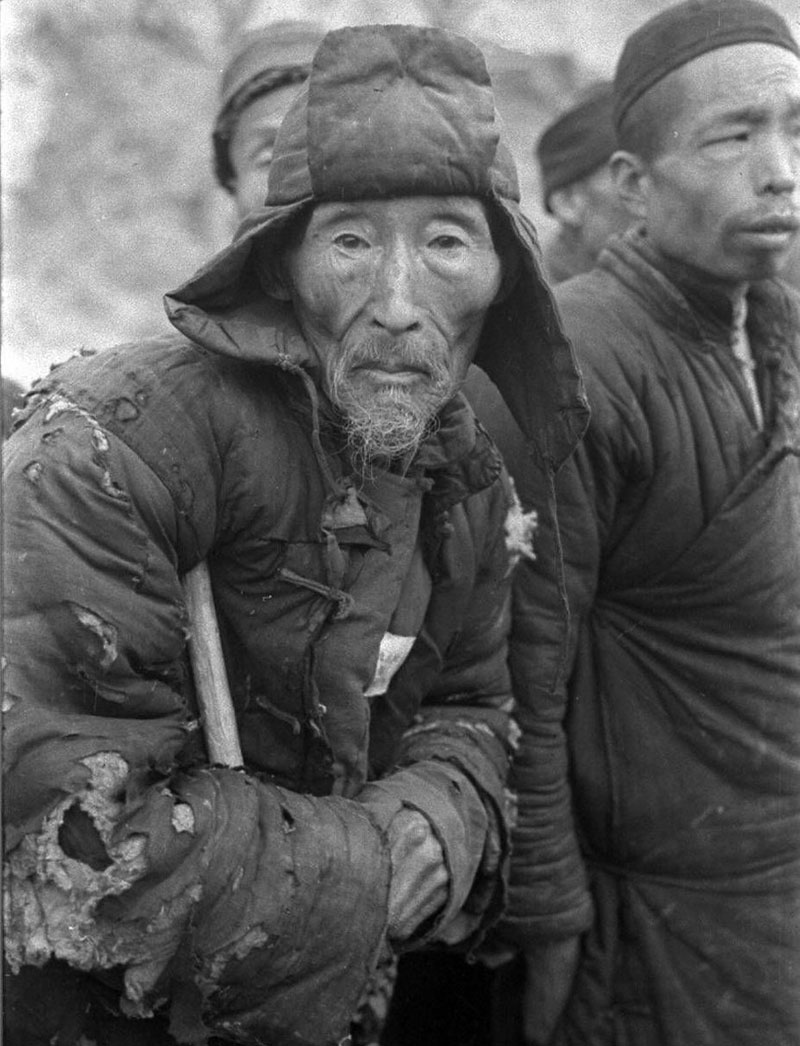
\includepdf[height=\paperheight]{Backmatter.jpg}
				\end{center}
			\end{figure}
\end{document}